%%%%%%%%%%%%%%%%%%%%%%%%%%%%%%%%%%%%%%%%%
% Masters/Doctoral Thesis 
% LaTeX Template
% Version 2.5 (27/8/17)
%
% This template was downloaded from:
% http://www.LaTeXTemplates.com
%
% Version 2.x major modifications by:
% Vel (vel@latextemplates.com)
%
% This template is based on a template by:
% Steve Gunn (http://users.ecs.soton.ac.uk/srg/softwaretools/document/templates/)
% Sunil Patel (http://www.sunilpatel.co.uk/thesis-template/)
%
% Template license:
% CC BY-NC-SA 3.0 (http://creativecommons.org/licenses/by-nc-sa/3.0/)
%
%%%%%%%%%%%%%%%%%%%%%%%%%%%%%%%%%%%%%%%%%

%----------------------------------------------------------------------------------------
%	PACKAGES AND OTHER DOCUMENT CONFIGURATIONS
%----------------------------------------------------------------------------------------

\documentclass[
11pt, % The default document font size, options: 10pt, 11pt, 12pt
oneside, % Two side (alternating margins) for binding by default, uncomment to switch to one side
spanish, % ngerman for German
singlespacing, % Single line spacing, alternatives: onehalfspacing or doublespacing
%draft, % Uncomment to enable draft mode (no pictures, no links, overfull hboxes indicated)
%nolistspacing, % If the document is onehalfspacing or doublespacing, uncomment this to set spacing in lists to single
%liststotoc, % Uncomment to add the list of figures/tables/etc to the table of contents
%toctotocnumbered, % Uncomment to add the main table of contents to the table of contents
parskip, % Uncomment to add space between paragraphs
%nohyperref, % Uncomment to not load the hyperref package
headsepline, % Uncomment to get a line under the header
chapterinoneline, % Uncomment to place the chapter title next to the number on one line
%consistentlayout, % Uncomment to change the layout of the declaration, abstract and acknowledgements pages to match the default layout
]{MastersDoctoralThesis} % The class file specifying the document structure


\selectlanguage{spanish}

\usepackage[utf8]{inputenc} % Required for inputting international characters
\usepackage[T1]{fontenc} % Output font encoding for international characters
\usepackage{float}
\usepackage{mathpazo} % Use the Palatino font by default

\usepackage[backend=biber,style=numeric,natbib=true,sorting=none]{biblatex} % Use the bibtex backend with the authoryear citation style (which resembles APA)

\addbibresource{references.bib} % The filename of the bibliography

\usepackage[autostyle=true]{csquotes} % Required to generate language-dependent quotes in the bibliography

\usepackage{tabularx}
\usepackage{dirtytalk}
\usepackage[document]{ragged2e}
\usepackage[final]{pdfpages}
\hyphenpenalty=9999
\exhyphenpenalty=9999


%----------------------------------------------------------------------------------------
%	MARGIN SETTINGS
%----------------------------------------------------------------------------------------

\geometry{
	paper=a4paper, % Change to letterpaper for US letter
	inner=2.5cm, % Inner margin
	outer=3.8cm, % Outer margin
	bindingoffset=.5cm, % Binding offset
	top=1.5cm, % Top margin
	bottom=1.5cm, % Bottom margin
	%showframe, % Uncomment to show how the type block is set on the page
}


%----------------------------------------------------------------------------------------
%	THESIS INFORMATION
%----------------------------------------------------------------------------------------

\thesistitle{DeltaML \\
Plataforma descentralizada de machine learning que preserva la privacidad del usuario} % Your thesis title, this is used in the title and abstract, print it elsewhere with \ttitle
\supervisor{Dr. Mariano \textsc{Beiró}} % Your supervisor's name, this is used in the title page, print it elsewhere with \supname
\examiner{} % Your examiner's name, this is not currently used anywhere in the template, print it elsewhere with \examname
\degree{Ingeniería en Informática} % Your degree name, this is used in the title page and abstract, print it elsewhere with \degreename
\author{
Fabrizio \textsc{Graffe} 93158\\
Agustín \textsc{Rojas}  91462
} % Your name, this is used in the title page and abstract, print it elsewhere with \authorname
\addresses{} % Your address, this is not currently used anywhere in the template, print it elsewhere with \addressname

\subject{Inform'\atica} % Your subject area, this is not currently used anywhere in the template, print it elsewhere with \subjectname
\keywords{} % Keywords for your thesis, this is not currently used anywhere in the template, print it elsewhere with \keywordnames
\university{\href{http://www.uba.ar}{Universidad de Buenos Aires}} % Your university's name and URL, this is used in the title page and abstract, print it elsewhere with \univname
\department{\href{http://www.fi.uba.ar}{Facultad de Ingenier\'ia}} % Your department's name and URL, this is used in the title page and abstract, print it elsewhere with \deptname
\group{\href{http://researchgroup.university.com}{Research Group Name}} % Your research group's name and URL, this is used in the title page, print it elsewhere with \groupname
\faculty{\href{http://www.fi.uba.ar}{Facultad de Ingenier\'ia}} % Your faculty's name and URL, this is used in the title page and abstract, print it elsewhere with \facname

\AtBeginDocument{
\hypersetup{pdftitle=\ttitle} % Set the PDF's title to your title
\hypersetup{pdfauthor=\authorname} % Set the PDF's author to your name
\hypersetup{pdfkeywords=\keywordnames} % Set the PDF's keywords to your keywords
}

\urlstyle{same}

\begin{document}

\frontmatter % Use roman page numbering style (i, ii, iii, iv...) for the pre-content pages

\pagestyle{plain} % Default to the plain heading style until the thesis style is called for the body content

%----------------------------------------------------------------------------------------
%	TITLE PAGE
%----------------------------------------------------------------------------------------

\begin{titlepage}
\begin{center}

\vspace*{.06\textheight}
{\scshape\LARGE \univname\par}
\vspace{0.7cm} % University name


\includegraphics[scale=0.3]{Logo} % University/department logo - uncomment to place it

\vspace{0.7cm} % University name


\textsc{\Large Informe de Trabajo Profesional}\\[0.5cm] % Thesis type

\HRule \\[0.4cm] % Horizontal line
{\huge \bfseries \ttitle\par}\vspace{0.4cm} % Thesis title
\HRule \\[1.5cm] % Horizontal line
 
\begin{minipage}[t]{0.4\textwidth}
\begin{flushleft} \large
\emph{Autores:}\\
{\authorname} % Author name - remove the \href bracket to remove the link
\end{flushleft}
\end{minipage}
\begin{minipage}[t]{0.4\textwidth}
\begin{flushright} \large
\emph{Tutor:} \\
{\supname} % Supervisor name - remove the \href bracket to remove the link  
\end{flushright}
\end{minipage}\\[3cm]

 
\vfill

{\large \today}\\[4cm] % Date

 
\vfill
\end{center}
\end{titlepage}

%----------------------------------------------------------------------------------------
%	LIST OF CONTENTS/FIGURES/TABLES PAGES
%----------------------------------------------------------------------------------------

\tableofcontents % Prints the main table of contents

%----------------------------------------------------------------------------------------
%	THESIS CONTENT - CHAPTERS
%----------------------------------------------------------------------------------------

\mainmatter % Begin numeric (1,2,3...) page numbering

\pagestyle{thesis} % Return the page headers back to the "thesis" style


\chapter{Introducci\'on}
\justify
El siguiente trabajo se presenta en el marco del desarrollo del Trabajo Profesional para la carrera Ingeniería en Informática de los estudiantes Fabrizio Sebastian Graffe y Agustín Rojas. 

El objetivo es aplicar los conocimientos adquiridos durante la carrera, por ésta razon se optó por desarrollar \textbf{\say{DeltaML: Plataforma descentralizada de machine \mbox{learning} que preserva la privacidad del usuario}}.

Machine learning (o \say{aprendizaje automático}) es una rama de la inteligencia artificial centrada en el estudio y construcción de sistemas capaces de aprender de los datos, identificar patrones y realizar decisiones con mínima intervención humana.

Blockchain \cite{bc} o DLT (Descentralized Ledger Technology), por su lado, es una tecnología que consta de un registro contable distribuido en una red de nodos. Este registro almacena las transacciones que se realizan entre los nodos de la red y cada uno tiene una copia completa. A su vez, para evitar que aquellos que sean maliciosos puedan cometer fraudes y/o alteraciones al registro, la tecnología cuenta con algoritmos de consenso y de prueba de trabajo realizado (Proof of Work).
Las ventajas de la tecnología Blockchain por sobre bases de datos tradicionales son:

\begin{itemize}
\item \textbf{Mayor transparencia:} Todas las transacciones son públicas, por lo que cualquier participante de la red puede verlas.
\item \textbf{Criptograficamente segura:} Debido a los algoritmos antes nombrados, para poder cometer fraude se necesitaría un poder de computo mayor al 51\% de la red (algo que no es posible hoy en día, al menos contra las redes de Bitcoin o Ethereum, ni por las mayores empresas de software en el mundo).
\item \textbf{Irreversibilidad:} Una transacción registrada en la blockchain no puede ser alterada por ninguno de los participantes de la red (otra vez, se necesitaría un poder de computo mayor al 51\% de la red).
\end{itemize}

\chapter{Descripci\'on del problema}

Tanto el área de Machine Learning como la tecnología Blockchain son elementos que están disrumpiendo la industria del software en la actualidad y tienen cada vez mas importancia en la vida diaria de las personas. En algunos casos su aplicación ha resultado en avances con un impacto positivo en la humanidad, pero también existen casos en los que se su impacto ha sido negativo.

Un ejemplo muy importante de mal uso de la tecnología es la red social Facebook, la cual ha tenido varios casos de violación de la privacidad de los datos de sus usuarios, venta e intercambio de éstos con otras compañías. Además del uso de técnicas de aprendizaje automático para generar adicción a las novedades en su plataforma y generación de cámaras de eco (echo chambers) por medio de filtrado de contenido \footnote{para mostrar a los usuarios solo opiniones similares a la suya, provocando así un refuerzo de su propia visión, aprovechándose de sesgos propios de los humanos como el Sesgo de Confirmación o Confirmation Bias}, por nombrar algunos.

Así como Facebook incurrió en estas malas prácticas que debilitan y manipulan a los usuarios de su plataforma, un abundante número de empresas e incluso estados también lo hacen a menudo.

La creciente necesidad de mantener la privacidad de nuestros datos, que día a día son mas valiosos, está provocando que diferentes gobiernos comiencen a plantear regulaciones mas estrictas en lo relativo al uso de los mismos.
Esto, a su vez, está impulsando una gran cantidad de iniciativas en el mundo para cambiar el paradigma actual, donde las empresas son dueñas de los datos de las personas, a uno donde las personas sean dueñas de sus propios datos y puedan venderlos para un uso determinado y ningún otro. En el ámbito local se tiene el ejemplo de Wibson como una empresa que va en ese camino. 

Teniendo en cuenta este contexto, se eligió la temática de este trabajo con la perspectiva de que en los años por venir se necesitarán maneras de entrenar modelos de Machine Learning que preserven la privacidad de las personas, es decir, sin que las empresas necesiten tener una copia de sus datos en sus bases de datos. Por lo cual el presente trabajo trata de contribuir en este paso hacia un futuro donde las personas sean dueñas de su información. 

\chapter{Estado del arte}

Actualmente existen varios proyectos en desarrollo y técnicas en investigación que intentan atacar la misma problemática de diferentes maneras.

\begin{itemize}
\item \textbf{Federated Learning: \cite{fedlearn2}} El aprendizaje federado es un método de aprendizaje automático en el que el objetivo es entrenar a un modelo centralizado de alta calidad con datos de entrenamiento distribuidos entre un gran número de clientes, cada uno con conexiones de red poco confiables y relativamente lentas. Los algoritmos de aprendizaje para esta configuración funcionan de la siguiente manera: en cada iteración, cada cliente calcula de forma independiente una actualización del modelo actual en función de sus datos locales y comunica esta actualización a un servidor central, donde las actualizaciones enviadas por los clientes se agregan para calcular una nueva versión global del modelo. Los clientes típicos en este entorno son los teléfonos móviles, y la eficiencia de la comunicación es de suma importancia. Actualmente, Google está investigando \cite{fedlearn1} \cite{fedlearn3} \cite{fedlearn4} \cite{fedlearn5} \cite{fedlearn6} esté método de aprendizaje automático y publicó varios papers al respecto, analizando mejoras y aplicaciones para dispositivos móviles (tales como predicción de palabras para GBoard).

\item \textbf{OpenMined: \cite{om}} Marketplace descentralizado de modelos de machine learning. Opera sobre la red de Ethereum. Utiliza Federated Learning para el entrenamiento de los modelos predictivos sobre Tensorflow y Pytorch ya que permiten entrenamiento desde clientes web. Modelos encriptados con homomorphic encryption \cite{homenc} para una transmisión de datos segura. 
Smart contracts regulan el marketplace y pagan a quienes gastaron poder de computo entrenando un proporcional de acuerdo a cuanto aportaron a la mejora del modelo global.
Actualmente en desarrollo.

\item \textbf{DML: \cite{dml}} Muy similar a OpenMined.

\item \textbf{NumerAI: \cite{nai}} Fondo de inversión que genera predicciones utilizando modelos predictivos crowd-sourced. Transforma y regulariza datos financieros en problemas de Machine Learning para ser resueltos por una red global de científicos de datos.

\item \textbf{Augur: \cite{aug}} Es un protocolo de predicción de mercados destinado a ser propiedad de las personas que lo usan.
Augur es un oráculo descentralizado y un protocolo peer to peer para la predicción de mercados. Augur es proyecto open-source. Es un conjunto de smart contracts escritos en Solidity que operan sobre Ethereum.


\item \textbf{Golem Network: \cite{gn}} Primera supercomputadora descentralizada que crea un marktplace global de poder de computo.
Golem conecta computadoras en una red peer-to-peer, permitiendo tanto a dueños de aplicaciones como a usuarios individuales ("requestors") alquilar recursos de las maquinas de otros usuarios ("providers"). Los pagos entre requestors, providers y desarrolladores de aplicaciones se realizan por medio de un sistema de transacciones basado en la red de Ethereum. 
El sistema está orientado a competir con los proveedores de infraestructura o servicios cloud para aplicaciones que requieran gran capacidad de computo reduciendo el precio de dicha capacidad. Como consecuencia, aplicaciones complejas como la representación CGI, el cálculo científico y el aprendizaje automático se volverían más accesibles.

\item \textbf{OceanProtocol: \cite{oc}} Ecosistema destinado a compartir activos y servicios. 
Los activos son datos y algoritmos. Los servicios son la integración, procesamiento, computación y almacenamiento. 
Ocean Protocol es un protocolo de intercambio de datos descentralizado, que permite que personas compartan y moneticen sus datos a la vez que garantiza control, auditabilidad, transparencia y conformidad a todos los actores involucrados.

\item \textbf{Wibson: \cite{wib}} Mercado de datos descentralizado, basado en blockchain, que proporciona a las personas una forma segura y anónima de vender información privada validada en un entorno confiable. Opera sobre la red de Ethereum. Las personas pueden vender sus datos por medio de la aplicación móvil de Wibson.
\end{itemize}

\chapter{Objetivos}
El presente trabajo consta de los siguientes objetivos principales:

\begin{itemize}
\item Desarrollar un marketplace de modelos de ML que permita a usuarios dueños de estos modelos entrenarlos de manera descentralizada preservando, al mismo tiempo, la privacidad de los datos que serán utilizados para dicho entrenamiento.
\item Desarrollar una forma de recompensar a los usuarios que provean datos y poder de computo para el entrenamiento de los modelos.
\item Desarrollar un framework de Federated Learning de código libre para generar un aporte a la comunidad.
\item Desarrollar un caso de uso de un modelo que requiera entrenamiento para hacer prueba del sistema desarrollado durante este trabajo.
\end{itemize}


\chapter{Introducción teórica}

\section{Machine Learning}
Machine Learning\cite{ml} o (Aprendizaje automático) es un subconjunto de la inteligencia artificial que se centra en el estudio y construcción de sistemas capaces de aprender de los datos, identificar patrones y realizar decisiones con mínima intervención humana.

Una definición más técnica podría ser: 

``\textit{Un programa aprende de la experiencia (\textbf{E}) con respecto a alguna tarea (\textbf{T}) y medida de desempeño (\textbf{P}), si su desempeño en dichas tareas mejora con la experiencia.}''

\textbf{Ejemplo:} un programa que aprende a jugar al ajedrez.
\begin{itemize}
\item \textbf{E} = la experiencia de jugar muchas partidas de ajedrez.
\item \textbf{T} = la tarea de jugar una partida de ajedrez.
\item \textbf{P} = la probabilidad de que el programa gane la próxima partida.
\end{itemize}

El programa que aprende de la experiencia, en el ámbito del aprendizaje automático es llamado \textbf{modelo}.


\subsection{Datasets}
Contiene las muestras (experiencias) necesarias para el proceso de aprendizaje y evaluación del modelo.
\begin{itemize}
\item \textbf{Set de entrenamiento:} muestras usadas para entrenar el modelo.
\item \textbf{Set de test:} muestras para evaluar cuán bien aprendió el modelo.
\end{itemize}

Si bien existen otros esquemas para separar el dataset y evaluar el modelo, se eligió éste al ser simple para no extender de más el alcance del trabajo.

\subsection{Entrenamiento y predicción}

Un modelo de aprendizaje automatico aprende de las experiencias o muestras dadas en forma de datos dentro del \textbf{Dataset}. Dicho proceso se dá como se describe a continación:

\subsubsection*{Entrenamiento}
\begin{itemize}
\item Se obtiene o genera el \textbf{dataset} (esto puede ser simple o puede contemplar la combinación de varias fuentes de datos).
\item Se realiza un \textbf{pre-proceso de los datos} contenidos en el dataset, de manera que puedan ser comprendidos y usados por el modelo en las etapas siguientes. Como ejemplo, los datos categoricos se codifican en valores numericos enteros o en variables dummy dependiendo de si sus valores tienen algun orden. 
\item Se divide el dataset en set de entrenamiento y set de test.
\item Se divide el set de entrenamiento en set de entrenamiento y set de validación.
\item Se \textbf{entrena el modelo} usando el set de entrenamiento.
\item Se \textbf{evalua el modelo} usando el set de validación.
\item Si la métrica de evaluación del modelo muestra que el modelo no cumple con la calidad requerida, se alteran los hiperparámetros del modelo y se lo vuelve a entrenar. 
\item Una vez que el modelo cumple con la calidad requerida segun las evaluaciones hechas contra el set de validación, se evalua el modelo contra el set de test y la métrica de calidad del modelo aquí obtenida es la que expresa que tan bien ha aprendido durante el proceso.
\item  Finalmente se obtiene el \textbf{modelo entrenado}.
\end{itemize}


\subsubsection*{Predicción}
\begin{itemize}
\item Se quiere realizar una predicción a partir de \textbf{un nuevo dato} del mismo tipo que los usados para entrenar y evaluar el modelo (es decir que, tiene los mismos features o atributos).
\item Se realiza un \textbf{pre-proceso del dato}, el mismo que se realizó para los datos de entrenamiento.
\item Se procede a darle esta nueva instancia de dato como entrada al \textbf{modelo}. La salida es la predicción hecha por el modelo entrenado.
\end{itemize}

\begin{figure}[H]
  	\centering
	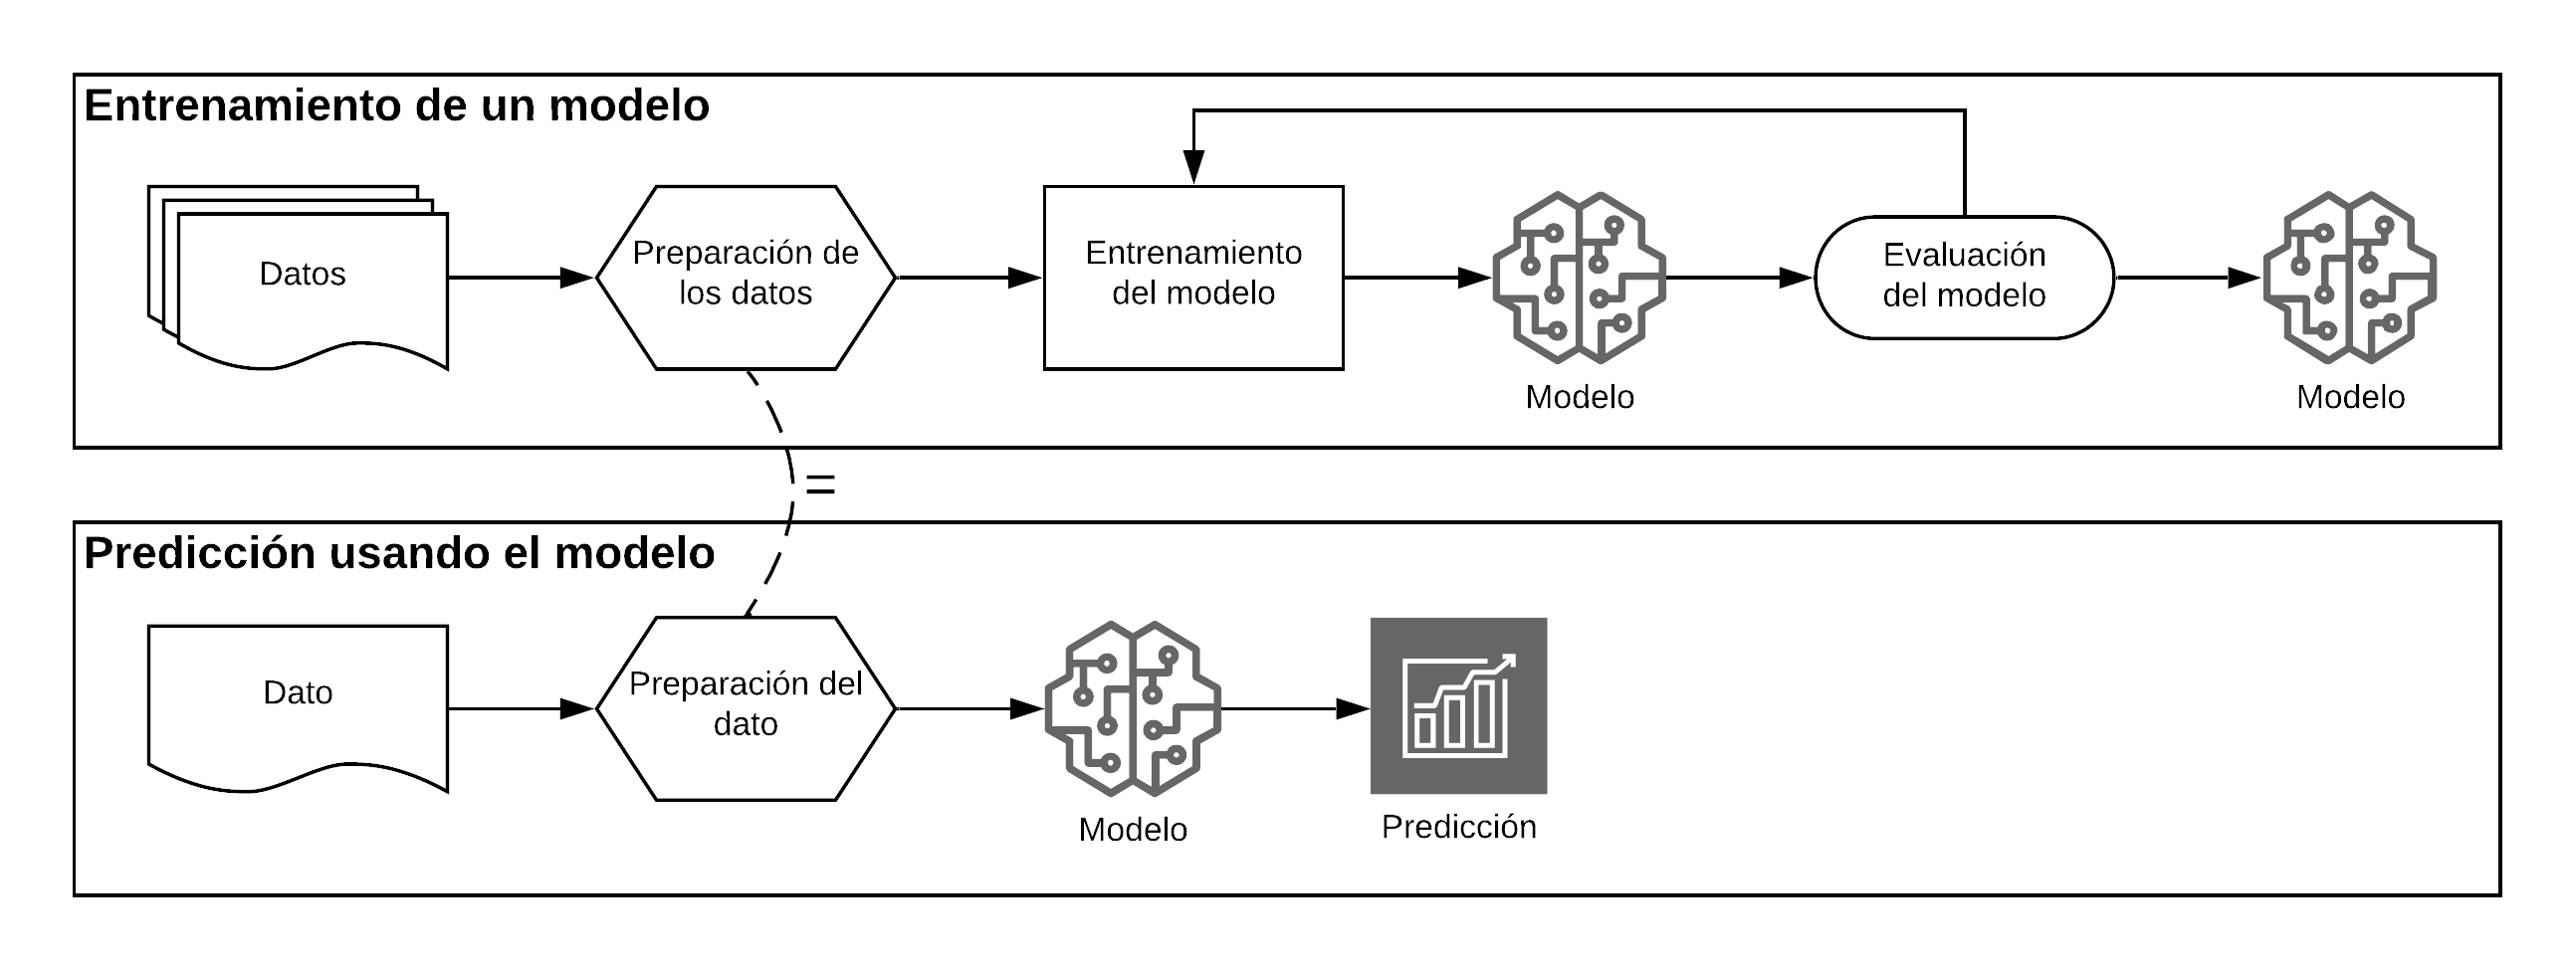
\includegraphics[scale=0.15]{imgs/ml-processes.png}
	\caption{Entrenamiento, evaluación y uso de un modelo de aprendizaje automático.}
\end{figure}

\subsection{Aprendizaje supervisado}
En el campo del aprendizaje automático, a los algoritmos que requieren de un conjunto de entrenamiento con datos etiquetados se denominan supervisados. Analizando estos ejemplos de entrenamiento, el sistema infiere funciones que pueden ser usadas para aplicarlas a nueva información.
Por el contrario, a los algoritmos que no son entrenados se los denomina no supervisados. Este grupo utiliza técnicas para encontrar patrones o grupos ocultos en los datos a analizar.


\section{SMPC (Secure Multi-party Computation)}
\justify
Una de las principales caracteristicas del presente trabajo es la posibilidad de realizar un c\'omputo entre varias partes de manera segura y privada, esto lleva el nombre de Secure Multi-party Computation. \\ 
Para ejemplificar, sean $P_{1},...,P_{n}$ diferentes partes dentro de un sistema distribuido, donde cada $P_{i}$ es dueño de un input $x_{i}$ y todas las partes están de acuerdo de usar una función $f$ que toma $n$ inputs. Su objetivo es computar $y = f(x_{1},...,x_{n})$ cumpliendo, al mismo tiempo, las siguientes condiciones:

\begin{itemize}
\item Exactitud (Correctness): el valor correcto de $y$ es computado.
\item Privacidad (Privacy): $y$ es la \'unica nueva informaci\'on que es publicada. Es decir, sus inputs siguen siendo secretos.
\end{itemize}

Existen muchos protocolos y m\'etodos para construir un sistema que asegure SMPC. Algunos de estos son:

\begin{itemize}{}
\item Protocolos basados en Homomorphic Encryption \ref{section-he}
\item Protocolos basados en zero proofs.
\end{itemize}

\section{Cifrado Asimétrico}
Es un método criptográfico que usa un par de claves para el envío de mensajes de manera segura. Ambas claves pertenecen a la persona que recibirá el dicho mensaje.
\begin{itemize}
\item \textbf{Clave pública:} que puede ser distribuida abiertamente
\item \textbf{Clave privada:} que solo conoce el propietario.
\end{itemize}
Cualquiera puede cifrar un mensaje usando la clave pública, pero ese mensaje cifrado sólo puede descifrarse con la clave privada.
Las claves se generan por medio de algoritmos basados en problemas matemáticos que no pueden ser resueltos por fuerza bruta en un tiempo razonable. 

\pagebreak

\section{Differential Privacy}
La privacidad diferencial \cite{diffpriv4} no es, en sí misma, una tecnología. Es una propiedad que describe algunos sistemas: una garantía matemática de que no se violará la privacidad uno o mas individuos si sus datos se utilizan para un determinado análisis. Un sistema que es diferencialmente privado permite realizar análisis sobre estos datos sensibles mientras los protege detrás de un velo de incertidumbre. \\
Otra definición \cite{diffpriv3} lo describe como una promesa hecha por aquellos individuos o entes que recaban o curan datos, a los due\~nos originales de los mismos. Dicha promesa expresa que la privacidad del dueño original no ser\'a afectada de forma adversa al permitir que sus datos sean usados en alg\'un estudio o an\'alisis, no importa qu\'e otros estudios, sets de datos o fuentes de informaci\'on haya disponibles.

\subsection{Local Differential Privacy}
Con la privacidad local, no hay una parte confiable; cada persona es responsable de agregar ruido a sus propios datos antes de compartirlos. Cada persona es un curador a cargo de su propia base de datos privada. Por lo general, un sistema privado local involucra a una parte no confiable (el agregador) que recopila datos de un gran grupo de personas a la vez.
La privacidad local es un modelo más conservador y seguro. Bajo la privacidad local, cada dato individual es extremadamente ruidoso y no es muy útil por sí solo. Sin embargo, en números muy grandes, el ruido de los datos se puede filtrar, y los agregadores que recopilan suficientes datos privados locales pueden hacer análisis útiles sobre las tendencias en todo el conjunto de datos.

\subsection{Global Differential Privacy}
Los sistemas privados a globales son generalmente más precisos: todo el análisis se realiza en datos "limpios", y solo se necesita agregar una pequeña cantidad de ruido al final del proceso. Sin embargo, para que funcione la privacidad global, todos los involucrados deben confiar en el curador. \\


\begin{figure}[H]
  	\centering
	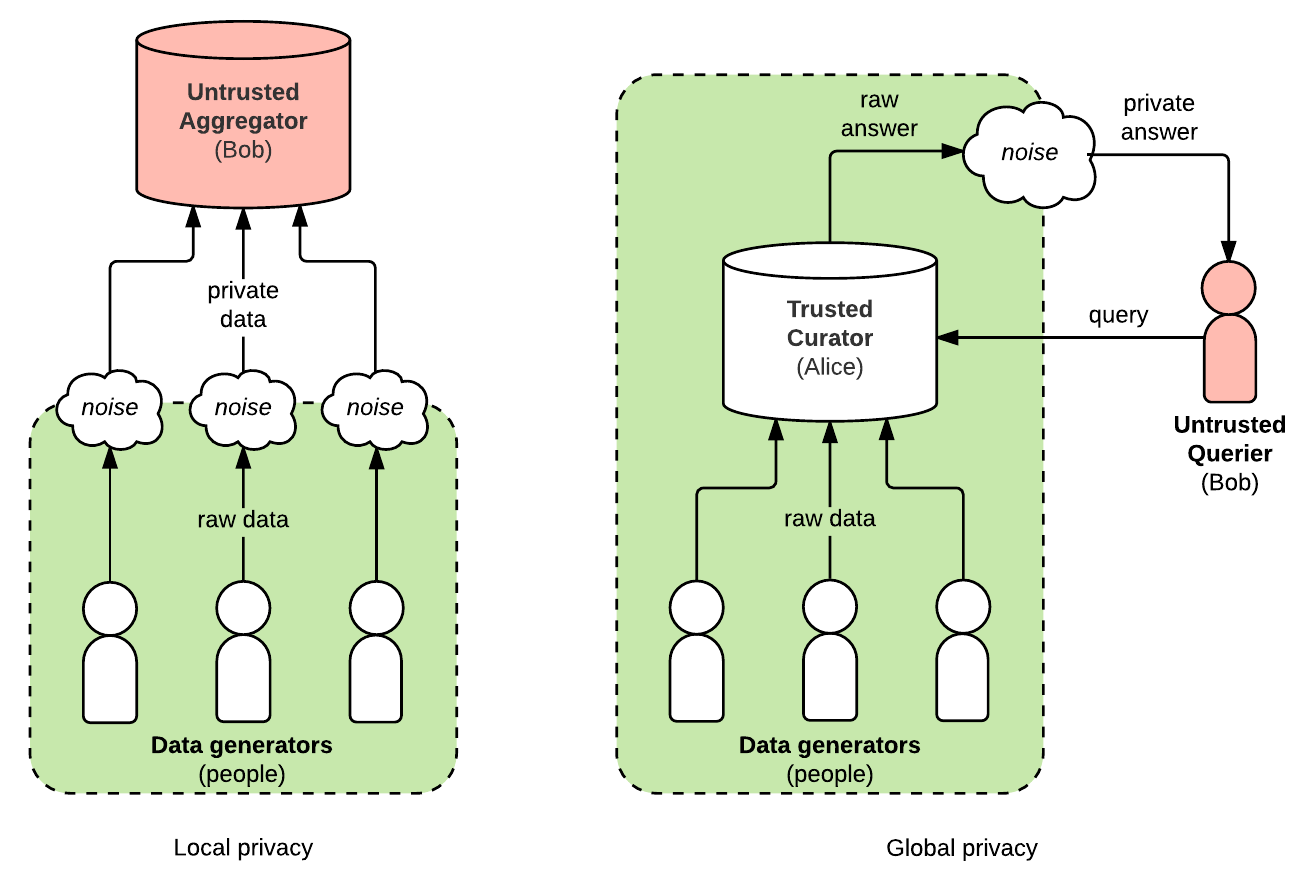
\includegraphics[scale=0.7]{imgs/diff-privacy.png}
	\caption{Local Differential Privacy vs. Global Differential Privacy}
\end{figure}



\chapter{Fundamentos y herramientas}

\section{Modelo de Regresión Lineal \cite{ml}}
Método estadístico que, en aprendizaje automático, se utiliza para predecir un valor objetivo (\textbf{y}) en base a variables independientes (los features o atributos, \textbf{X}).

$ x_{j}^{(i)} $ = el valor del feature j en la i-ésima muestra de entrenamiento \\
$ x^{(i)} $ = los features de la i-ésima muestra de entrenamiento \\
$ m $ = la cantidad de muestras de entrenamiento \\
$ n $ = el número de features 

El modelo de regresión tiene la forma expresada en la ecuación \ref{eq:1}

\begin{equation}
h_{w}(x) = w_{o} + w_{1}x_{1} + w_{2}x_{2} + w_{3}x_{3} + ... + w_{n}x_{n} \label{eq:1}
\end{equation}

\subsection*{Función de costo}
Expresa qué tanto error está cometiendo el modelo actualmente al predecir para cada una de las muestras del dataset.

\textbf{Mean Squared Error} (Error cuadrático medio)
\begin{equation}
MSE = \frac{1}{m} \sum_{i=1}^{m} (h(x^{(i)}) - y^{(i)})^2
\end{equation} 

\subsection*{Gradient Descent}
Algoritmo de optimización iterativo para hallar el mínimo de una función. Se utiliza, en el contexto del entrenamiento de un modelo de regresión lineal, para hallar los pesos \textbf{w} (parámetros del modelo de regresión lineal).

Repetir hasta que converja:
\begin{equation}
w_{j} = w_{j} - (\frac{\alpha}{m} \sum_{i=1}^{m} (h_{w}(x)^{(i)} - y^{(i)}) \cdot x_{j}^{(i)} para j := 0...n
\end{equation}


\pagebreak

\section{Homomorphic Encryption}\label{section-he}
\cite{homenc} Método de encriptación asimétrico que permite realizar cálculos directamente sobre datos encriptados sin requerir acceso a la clave privada. El resultado de tal cálculo permanece en forma encriptada, y puede ser revelado posteriormente por el propietario de la clave.

\begin{figure}[H]
  	\centering
	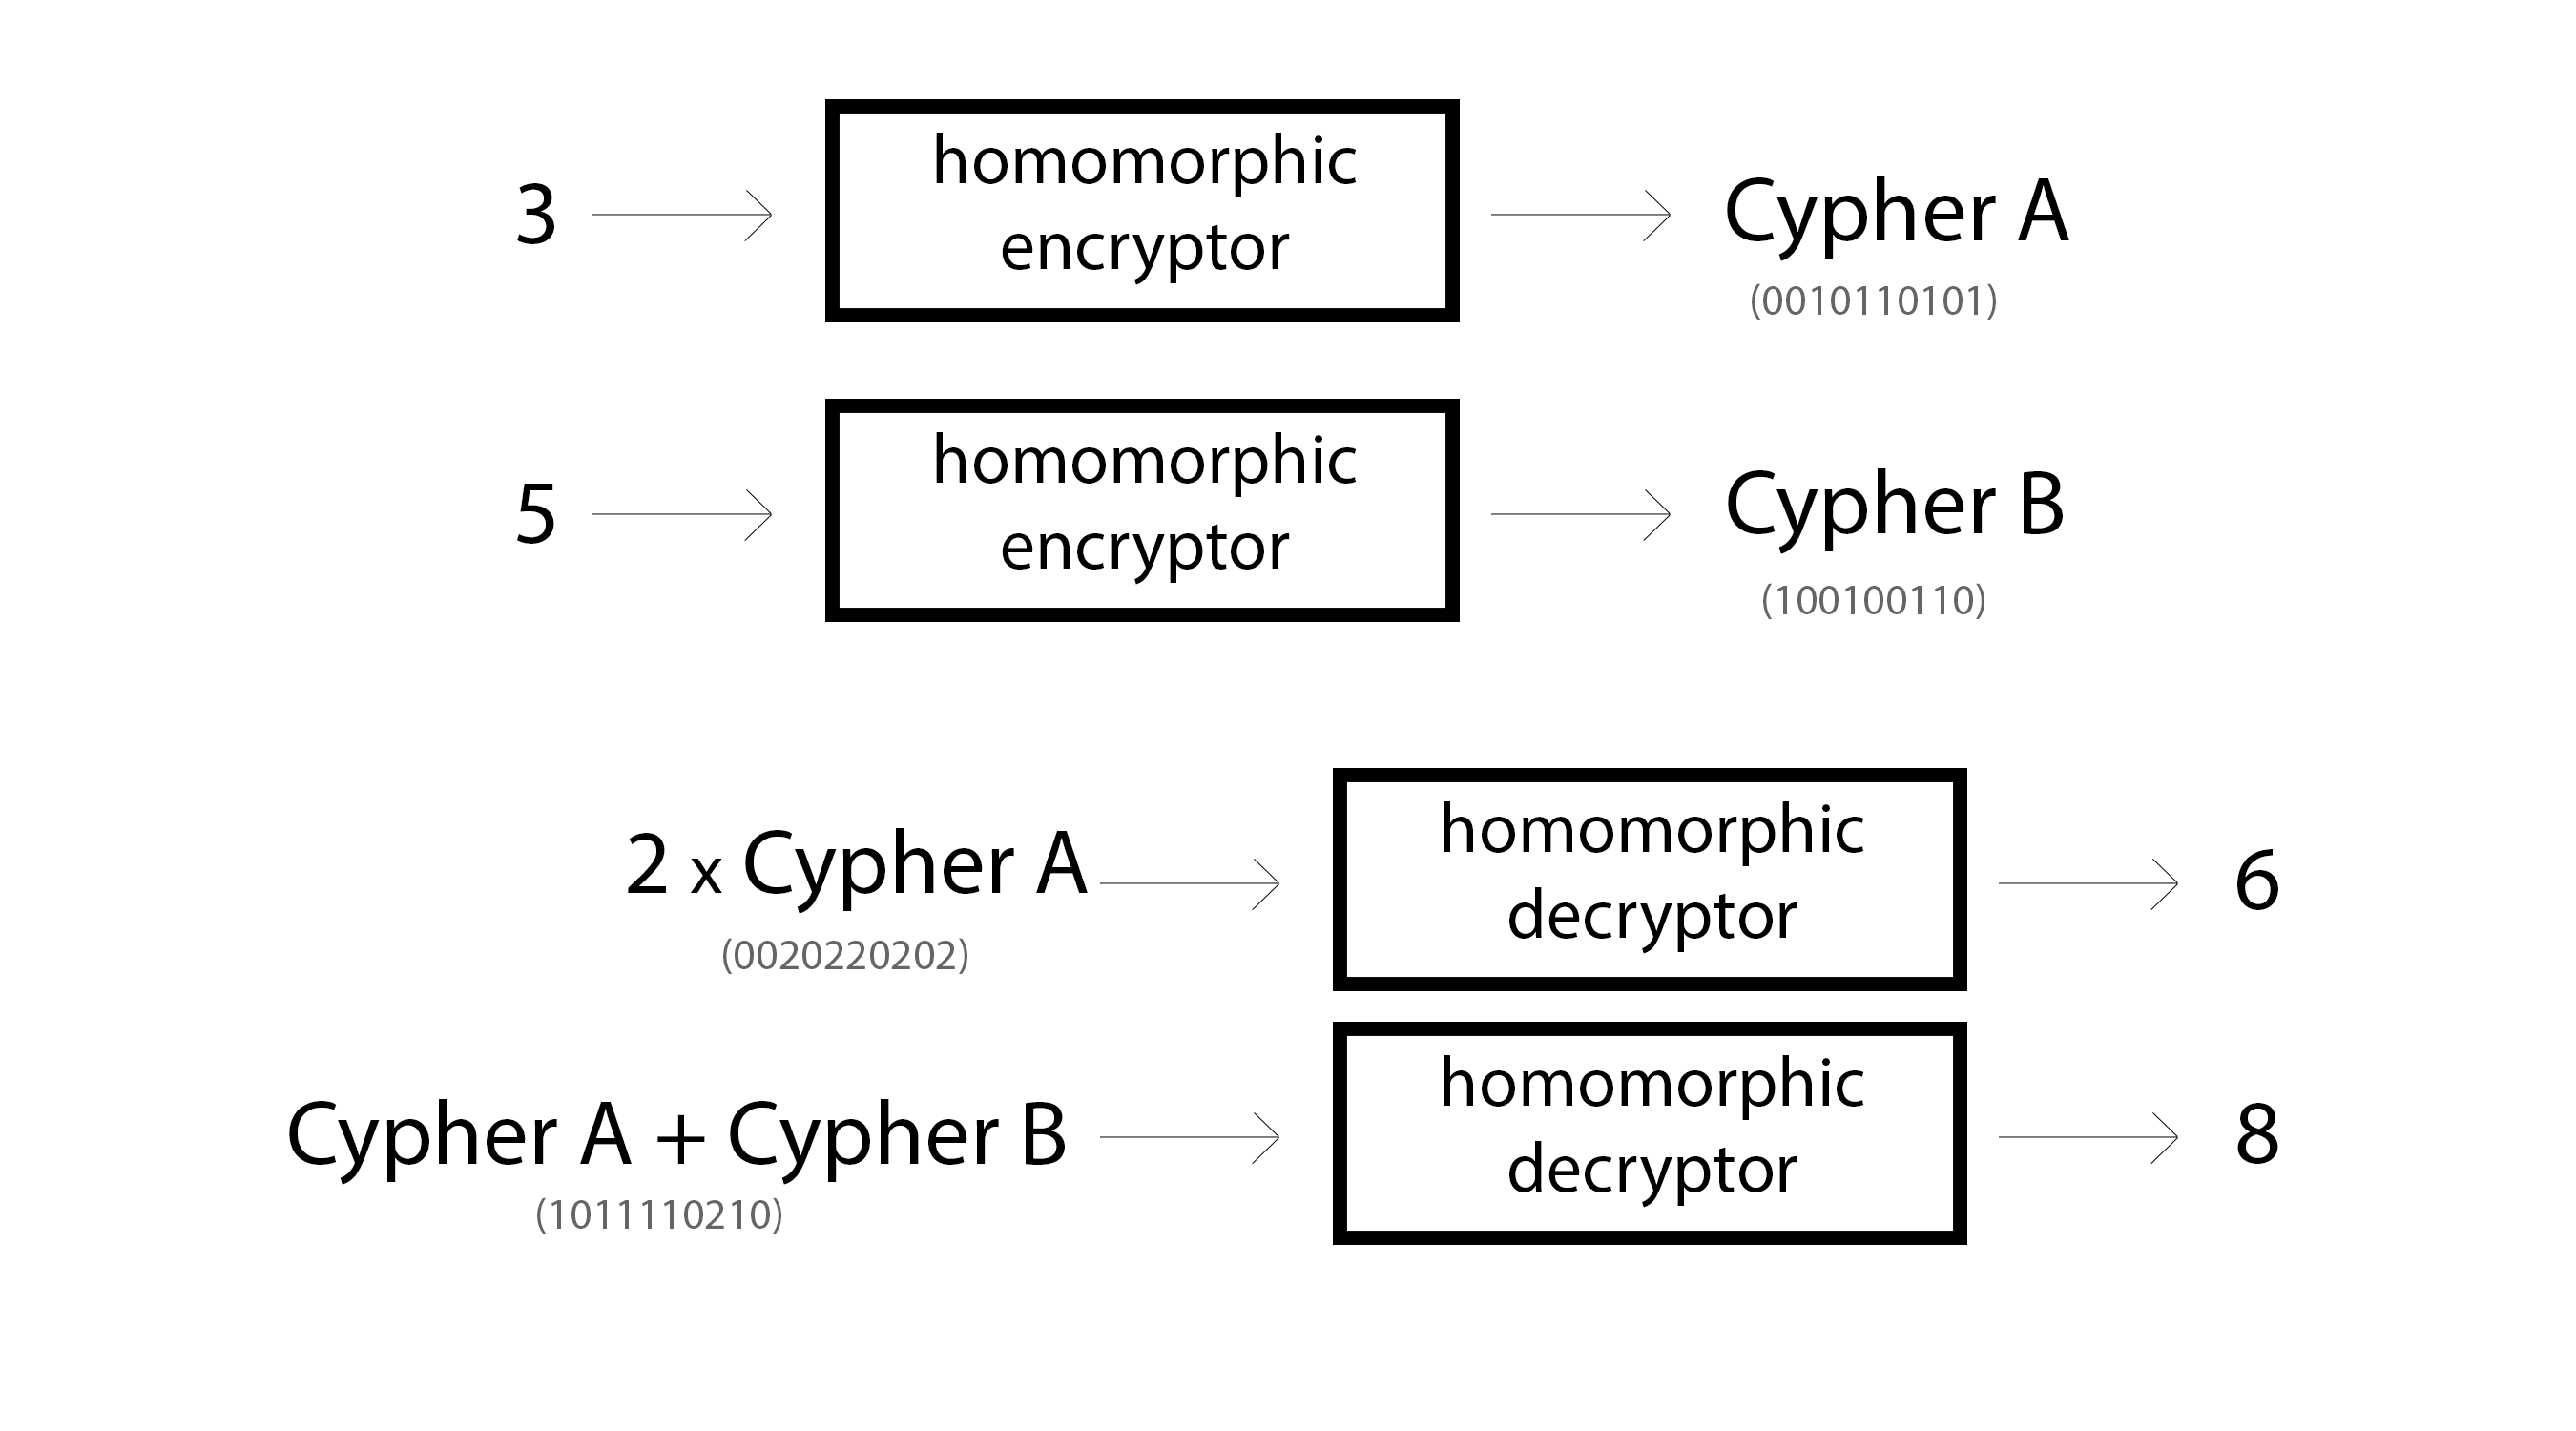
\includegraphics[scale=0.5]{imgs/he.png}
	\caption{\cite{he} Ejemplos de operaciones matemáticas realizadas sobre números encriptados por medio de Homomorphic Encryption.}
\end{figure}

Dentro de los cifrados con propiedades homomorficas, se pueden distinguir dos tipos \cite{homenc1} \cite{homenc2}: Fully Homomorphic Encryption y Partially Homomorphic Encryption.

\subsection*{Fully Homomophic Encryption}
Un cifrado se considera totalmente homomórfico si exhibe tanto homomorfismo\footnote{\textbf{Homomorfismo en encriptación}: propiedad en la cúal luego de realizar una operación algebraica con los datos cifrados, al desencriptar el resultado de la misma se obtiene el mismo resultado que si ésta se hubiera realizado sobre los datos sin cifrar.} aditivo como multiplicativo.

\subsection*{Partially Homomophic Encryption}
Un cifrado es considerado parcialmente homomórfico si exhibe homomorfismo aditivo o multiplicativo, pero no ambos. Algunos ejemplos de estos sistemas son:
\begin{itemize}
\item \textbf{RSA:} homomorfismo multiplicativo. 
\item \textbf{ElGamal:} homomorfismo multiplicativo.
\item \textbf{Paillier:} homomorfismo aditivo.
\end{itemize}

\subsubsection*{Paillier}
El criptosistema utilizado en este trabajo es uno basado en Paillier \cite{paillier}. 
Las propiedades homomorficas de un sistema de encriptación del tipo paillier son:

\begin{itemize}
\item Números encriptados pueden ser multiplicados por un escalar no encriptado.
\item Números encriptados pueden ser sumados entre sí.
\item Numeros encriptados pueden ser sumados a escalares no encriptados.
\end{itemize}

Se optó por éste cripto-sistema por la facilidad que brinda una de sus implementaciones (python-paillier) para la serialización y deserialización de números encriptados. 

\section{Federated Learning}
El aprendizaje federado \cite{fedlearn2} \cite{fedlearn1} \cite{fedlearn3} \cite{fedlearn4} \cite{fedlearn5} \cite{fedlearn6} es un método de aprendizaje automático en el que el objetivo es entrenar a un modelo centralizado de alta calidad con datos de entrenamiento distribuidos entre un gran número de clientes, cada uno con conexiones de red poco confiables y relativamente lentas. Los algoritmos de aprendizaje para esta configuración funcionan de la siguiente manera: en cada iteración, cada cliente calcula de forma independiente una actualización del modelo actual en función de sus datos locales y comunica esta actualización a un servidor central, donde las actualizaciones enviadas por los clientes se agregan para calcular una nueva versión global del modelo.

\begin{figure}[H]
  	\centering
	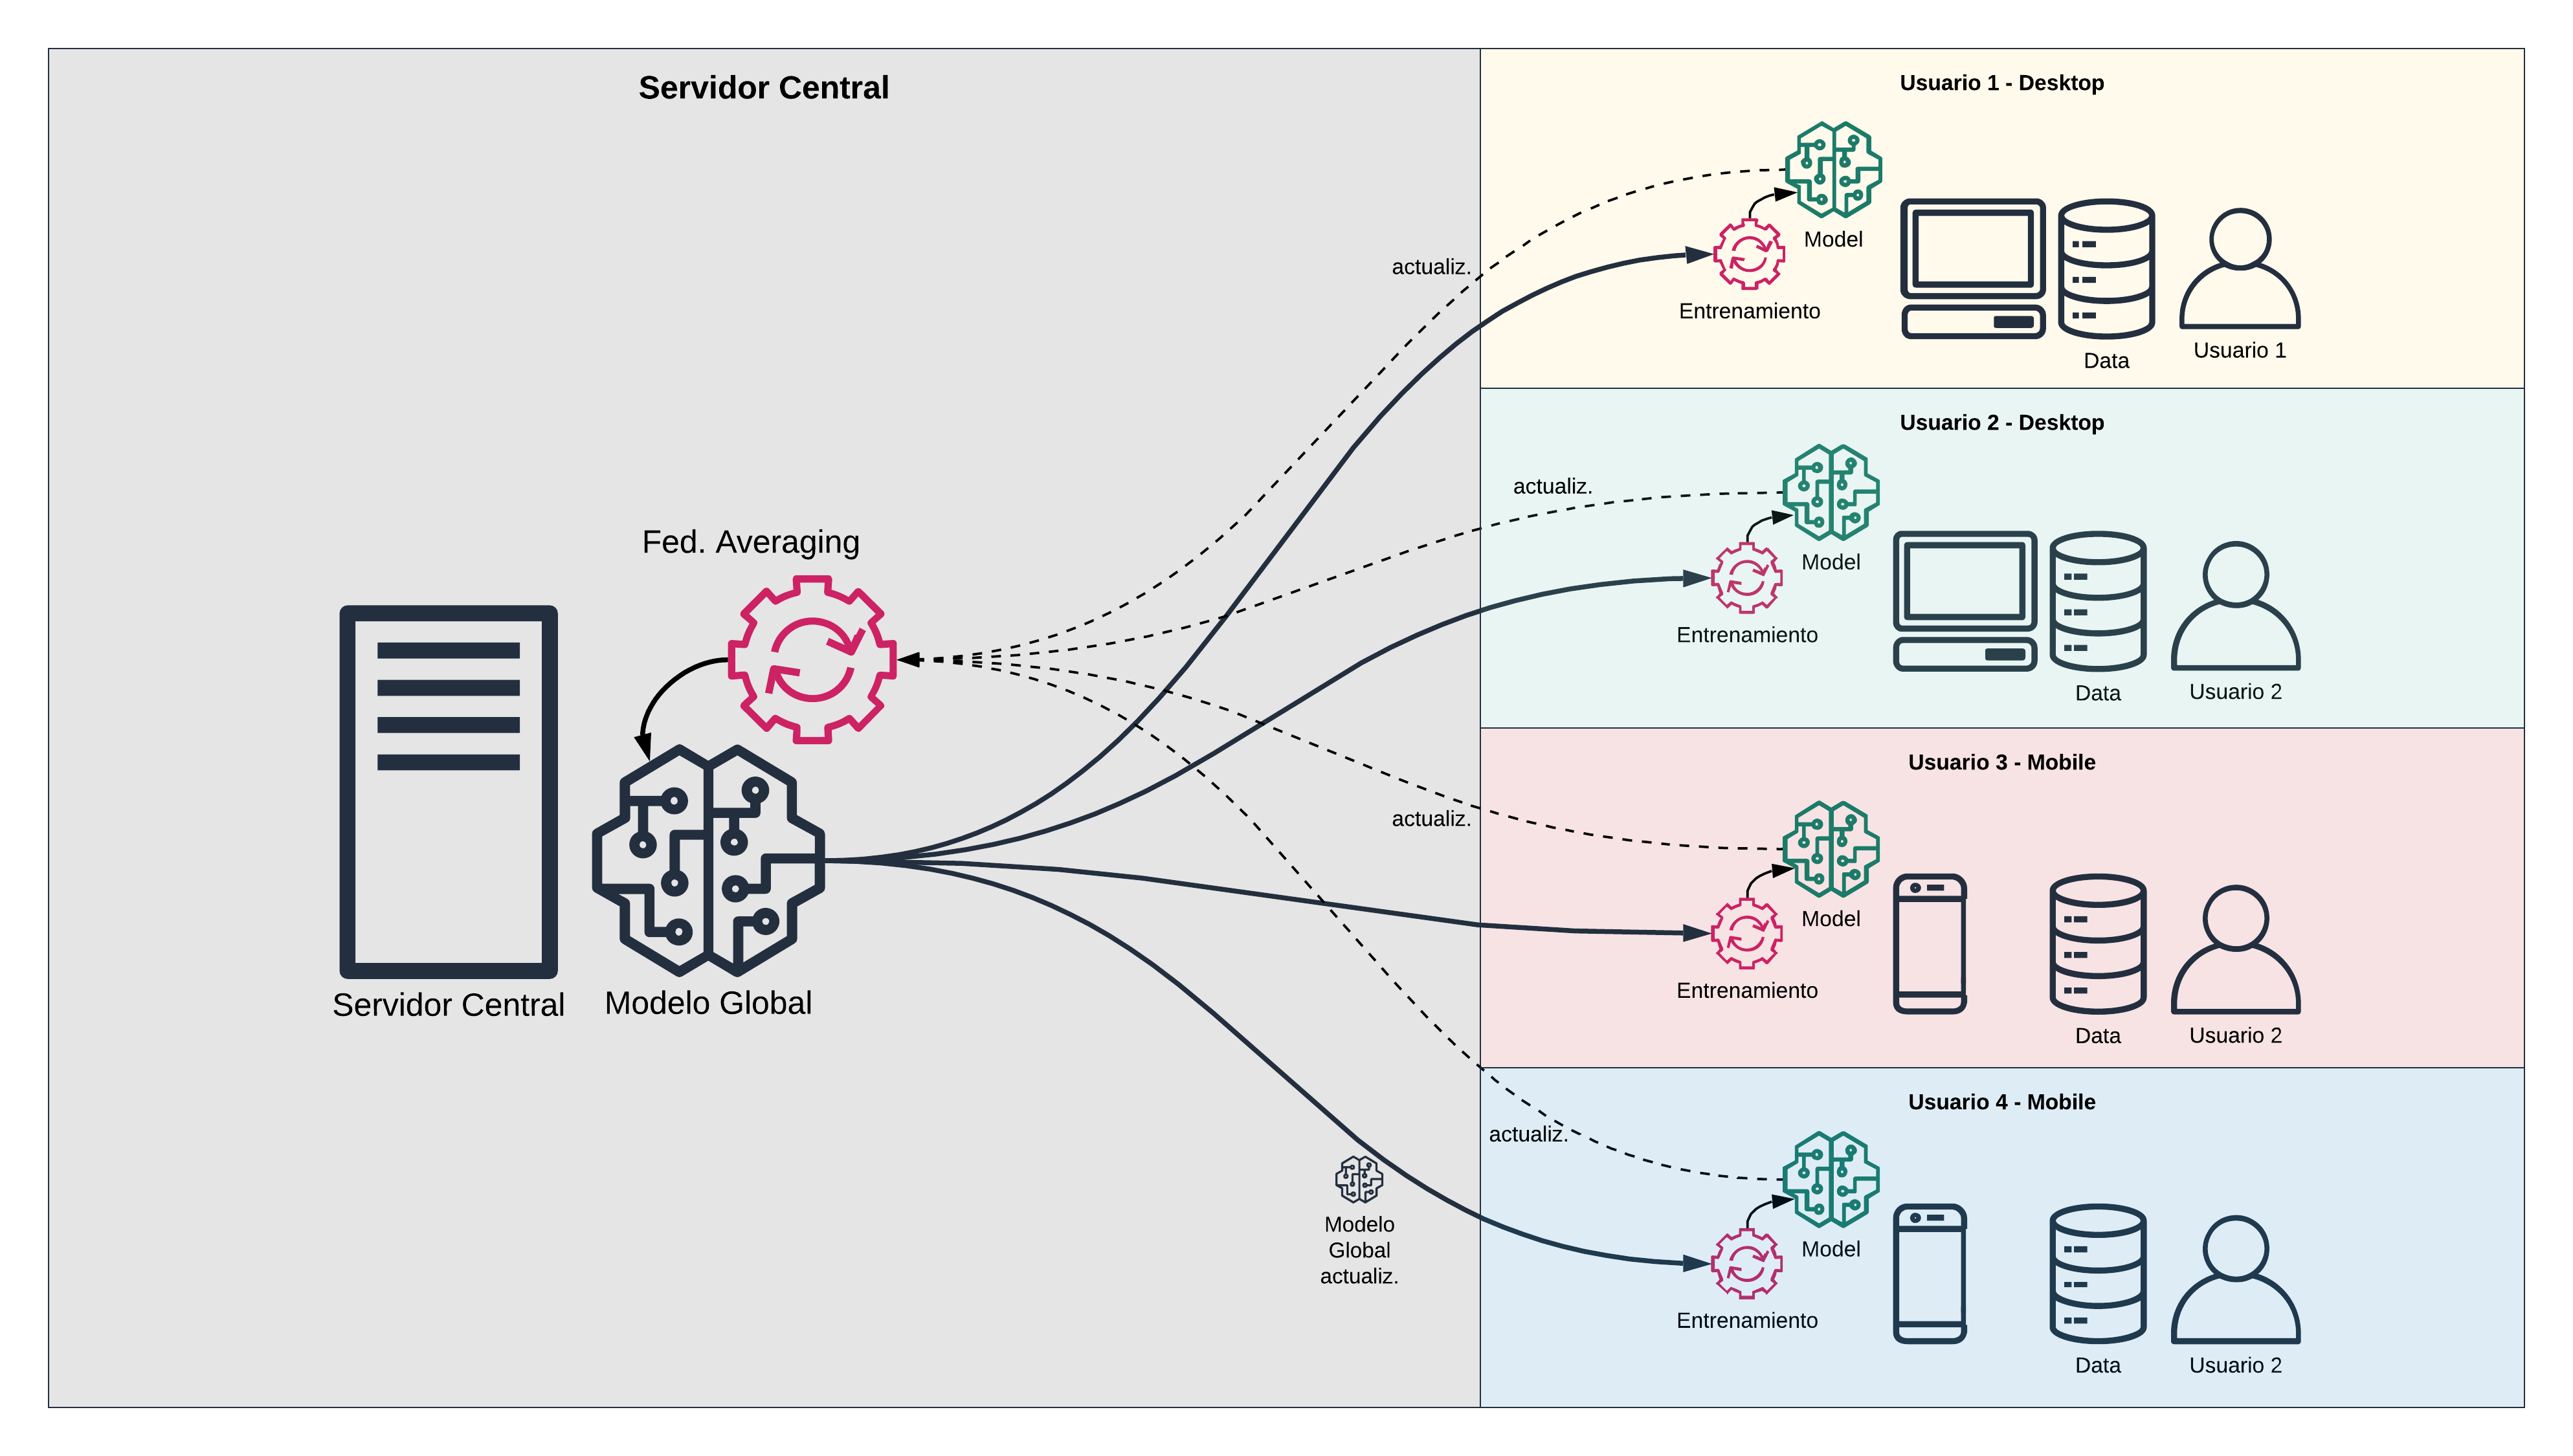
\includegraphics[scale=0.42]{imgs/fl_flow.png}
	\caption{Esquema de entrenamiento de un modelo usando Federated Learning.}
\end{figure}

\subsection*{Caracteristicas}
\begin{itemize}
\item Los clientes eligen si participan en el entrenamiento. 
\item El número de clientes disponible puede ser grande y variable.
\item Incorpora preservación de la privacidad por medio de entrenamientos distribuidos.
\item Los datos en general no están balanceados, ya que son específicos del cliente y auto-correlacionados.
\end{itemize}


\section{Blockchain \cite{bc}}

\textit{Blockchain es un registro contable abierto y distribuido que puede registrar transacciones entre dos partes eficientemente y de forma verificable y permanente.}\cite{bc-def} \\

Este registro contable distribuido está tipicamente administrado por una red peer-to-peer que adhiere colectivamente a un protocolo para la comunicación entre nodos y validación de nuevas transacciones.
Una Blockchain está compuesta por las siguientes partes:

\textbf{Registro contable digital} donde se anotan todas las transacciones agrupadas en bloques. \\
\textbf{Las billeteras digitales o wallets}, permiten a los usuarios realizar transacciones y manejar sus identidades digitales. \\
\textbf{Los mineros}, generan nuevos bloques (con las transacciones iniciadas por los usuarios de la red) resolviendo un problema matemático del protocolo de consenso. Reciben una recompensa por su trabajo. \\
\textbf{Los nodos}, almacenan una copia exacta del libro contable y validan nuevos bloques.

Se puede observar en la figura \ref{fig:bc-exp} una explicación del proceso que se dispara al realizarse una nueva transacción. 

\subsubsection*{Caracteristicas}
\begin{itemize}
\item \textbf{Pseudónimo}: ya que los usuarios se identifican por medio de direcciones que no pueden ser relacionadas directamente con ellos sin alguna información externa.
\item \textbf{Irreversible e inmutable}: Los bloques que ya se hayan agregado a la cadena no pueden ser alterados ni borrados ya que cada uno tiene una referencia al anterior, todos los nodos validan constantemente la cadena y los nuevos bloques que se agregan a ella por medio de algoritmos de consenso.
\item \textbf{Descentralizado}: Todos los participantes de la red tienen una copia de la cadena de bloques y no está controlada por una sola entidad por lo que no hay un punto único de fallo.
\item \textbf{Consensuado}: Por medio de algoritmos de consenso que aprovechan la descentralización, se evitan fraudes y ataques.
\item \textbf{Cronología:} Cada bloque tiene información del momento en el que fue creado y cual fue su bloque anterior.
\item \textbf{Transparencia:} Todos los participantes de la red pueden ver el historial transacciones que se ejecutaron hasta el momento y los bloques que las contienen.
\end{itemize}

\begin{figure}[H]
  	\centering
	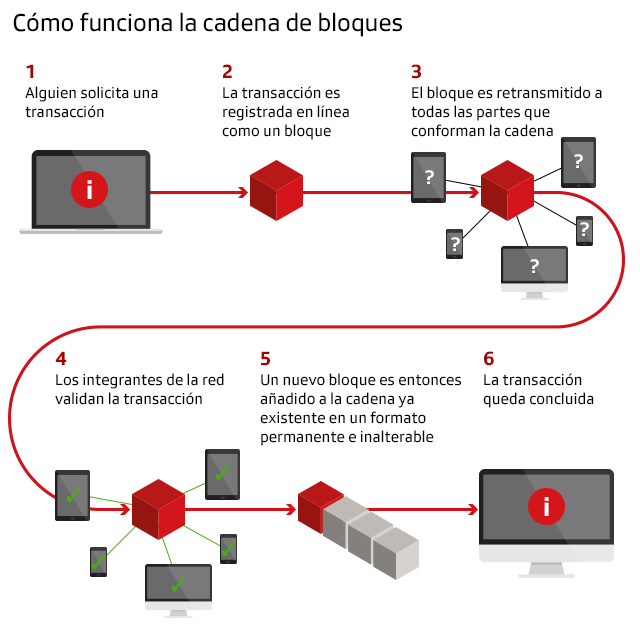
\includegraphics[scale=0.5]{imgs/blockchain-explained.png}
	\caption{Cómo se procesa una nueva transacción en la Blockchain. \\ \textbf{Fuente:} Financial Times / PwC United States}
	\label{fig:bc-exp}
\end{figure}

\subsection{Smart Contracts \cite{sc}}
Aplicación informática que se programa para que ejecute acuerdos que hayan determinado dos o más partes de forma automática y sin necesidad de que un juez o una autoridad exija su cumplimiento.
Queda almacenado en la Blockchain y por lo tanto cumple con las mismas características que se mencionaron antes.
Un Smart Contract consta consta de las siguientes partes:

\begin{itemize}
\item \textbf{Address:} Una dirección donde se encuentra desplegado el contrato. Las partes usan esta dirección para interactuar con él.
\item \textbf{Código:} El contrato inteligente necesita que los acuerdos entre las partes esten escritos en forma de código. En general, se utiliza Solidity como lenguaje de programación. Adicionalmente, al compilar el código del contrato, se genera el binario de este para ser desplegado a la red de nodos (en este caso, Ethereum) y, lo que se llama ABI (Application Binary Interface), que no es más que la interfaz que deben conocer las aplicaciones que quieran comunicarse con dicho contrato.
\item \textbf{Estado:} Los diferentes eventos o mensajes que le lleguen al contrato modificaran su estado interno (dependiendo de la lógica que se le haya programado).
\item  \textbf{Balance:} El contrato es capaz de almacenar dinero (en forma de Ether para la Blockchain Ethereum), y distribuirlo segun la lógica que se le haya programado.
\end{itemize}


\newpage

\chapter{Implementación}

\section{DeltaML: Interacción entre participantes}
En la figura \ref{fig:interact} se observa se observa un diagrama del sistema y las diferentes interacciones entre los participantes.

\begin{figure}[H]
  	\centering
	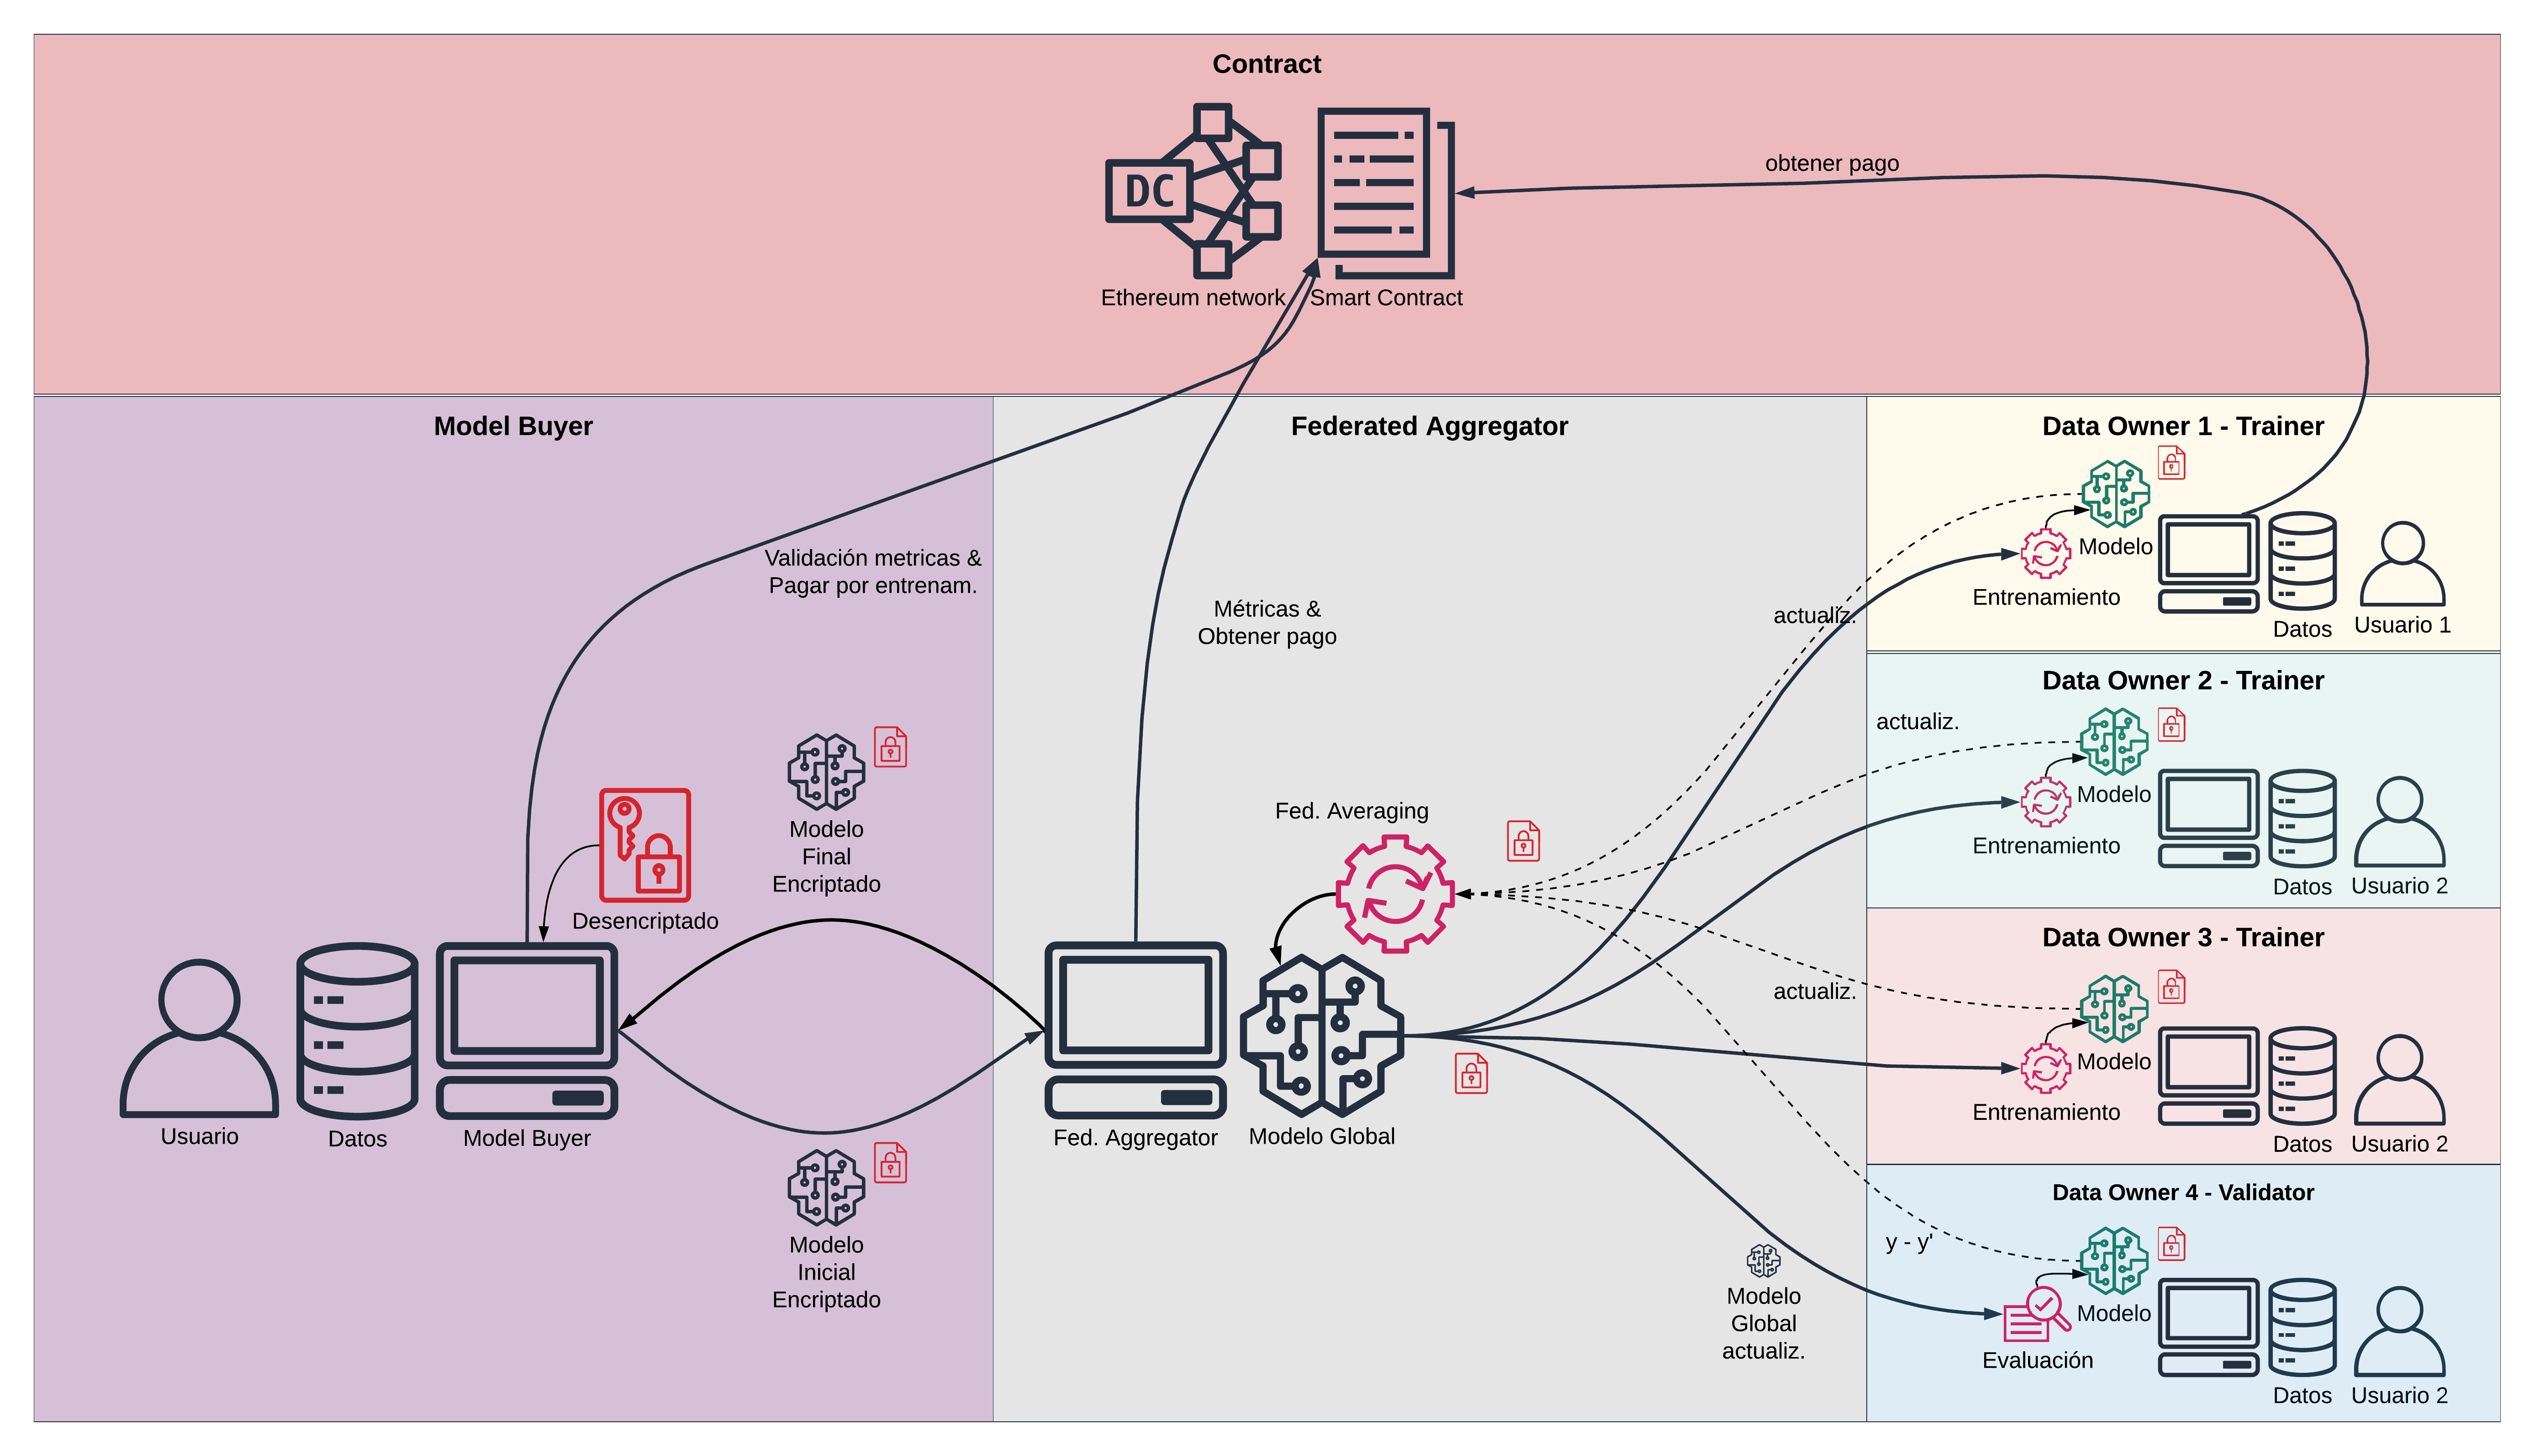
\includegraphics[scale=0.072]{imgs/deltaml_flow.png}
	\caption{Interacciones de los módulos del sistema}
	\label{fig:interact}
\end{figure}

\begin{enumerate}
\item El Model Buyer solicita a la plataforma el entrenamiento de un determinado modelo usando datos que cumplan ciertos requerimientos. El Model Buyer entonces envía un modelo encriptado sin entrenar al Federated Aggregator e inicializa una transacción de modelo en el smart contract.
\item Previamente, varios Data Owners se registraron al Federated Aggregator y en el smart contract para estar disponibles a nuevas solicitudes de entrenamientos.
\item El Federated Aggregator les envía la solicitud de entrenamiento a cada uno de los Data Owners registrados así como también los requerimientos sobre los datos.
\item Cada Data Owner debe asegurarse de tener los datos requeridos, luego de lo cual, si así lo desean, aceptan la solicitud de participación en el entrenamiento.
\item El Federated Aggregator les asigna un rol de entrenador o validador a cada uno de los Data Owners, y les envía el modelo inicial encriptado.
\item Para el caso de un entrenamiento de un modelo de regresión lineal (el caso implemenentado en este trabajo), cada Data Owner con rol de entrenador realiza N pasos de Gradient Descent de manera local con sus datos privados, y envía el modelo actualizado encriptado, luego de este proceso, al Federated Aggregator.
\item El Federated Aggregator realiza un promedio de todas las actualizaciones encriptadas, actualiza el modelo global que mantiene (también encriptado) y lo vuelve a enviar a los Data Owners para repetir el proceso.
\item El Federated Aggregator al finalizar el entrenamiento actualiza las métricas de calidad del modelo en el smart contract.
\item El model buyer recibe el modelo entrenado, y verifica las métricas de calidad en el smart contract usando el protocolo explicado en la figura \ref{fig:flujo_valid}.
\item El smart contract calcula las contribuciones de los participantes y realiza los pagos correspondientes por el entrenamiento y validacion del modelo.
\end{enumerate}


\section{Data Owner}
\justify
El Data Owner es aquel que ejecuta en su computador el cliente web por medio del cual puede decidir en qué solicitudes de entrenamiento participar. Tiene en su poder uno o mas datasets. Es recompensado por su contribución al entrenamiento de un modelo, ya sea su rol validador o entrenador. En el caso de que su rol sea entrenador, la recompensa es proporcional a lo contribuido a la mejora de la calidad del modelo. En cambio, para su rol como validador, recibe una recompensa fija que no depende de cuanto haya mejorado este.

\subsection*{Capacidades}
\begin{itemize}
\item Elige participar en el entrenamiento de un modelo.
\item Aporta sus datos para, de manera local y sin poder ver el modelo.
\item Entrenar el modelo solicitado por el Model Buyer.
\item Calcular diferencia entre predicciones del modelo y lo esperado.
\end{itemize}

\subsection*{Limitaciones}
No puede:
\begin{itemize}
\item Ver los parámetros del modelo en entrenamiento, trabaja con el modelo encriptado.
\item Alterar el cálculo de las métricas de calidad o su contribución para ganar más dinero por el entrenamiento. 
\end{itemize}

\subsection*{Roles}
\begin{itemize}
\item \textbf{Trainer:} Usa sus datos privados y su poder de cómputo para entrenar modelos.
\item \textbf{Validator:} Usa sus datos privados y su poder de cómputo para  calcular diferencias entre lo esperado y las predicciones.
\end{itemize}

Los Data Owners se dividen en Trainers y Validators en proporciones de 70\% y 30\% respectivamente tal como se haría con un dataset en sets de entrenamiento y test. Queda para futuros desarrollos realizar una mejora utilizando un K-Fold Cross-validation.


\section{Model Buyer}
\justify
El Model Buyer interactua con el sistema por medio del marketplace, publicando una solicitud de entrenamiento para un cierto modelo con ciertas caracteristicas.
Al crear la solicitud envía un modelo inicial encriptado con Homomorphic Encryption al Federated Aggregator junto con  las carácteristicas que debe cumplir el dataset para entrenar el modelo. 
Al mismo tiempo, inicializa en un smart contract desplegado en la red Ethereum, la transacción del correspondiente al entrenamiento del modelo y envía el monto que destina al proceso de mejorar el modelo inicial, las metricas de calidad del modelo inicial y los participantes involucrados.

\subsection*{Capacidades}
\begin{itemize}
\item Solicita el entrenamiento de un modelo.
\item Paga por el modelo entrenado.
\item Desencripta el modelo una vez entrenado.
\item Valida métricas de calidad del modelo.
\end{itemize}

\subsection*{Limitaciones}
No puede:
\begin{itemize}
\item Ni ver ni robar los datos con los que se entrenan los modelos.
\item Alterar las métricas de calidad del modelo.
\item Realizar fraude en el pago por el modelo.
\end{itemize}



\section{Federated Aggregator}
Este participante del sistema actúa como orquestador de los diferentes entrenamientos distribuidos y como mediador entre los Data Owners y Model Buyer. Para lograr una verdadera descentralización se necesitaría tener varios participantes de la plataforma actuando como Federated Aggregators.

\subsection*{Capacidades}
\begin{itemize}
\item Asigna roles a los Data Owners que participan en un entrenamiento.
\item Agrega de manera segura las actualizaciones al modelo provenientes de cada Data Owner.
\item Envía el modelo actualizado encriptado a los Data Owners para que continúen el entrenamiento.
\item Calcula las métricas de calidad del modelo.
\end{itemize}

\subsection*{Limitaciones}
No puede:
\begin{itemize}
\item Robar el modelo en entrenamiento, está encriptado.
\item Alterar el cálculo de las métricas de calidad ni las contribuciones de cada Data Owner (las valida el Model Buyer).
\end{itemize}


\section{Contract}
El smart contract es el encargado de regular el mercado, recibe solicitudes provenientes del Model Buyer y las vincula con los Data Owners que las acepten y al modelo en entrenamiento. Al mismo tiempo, permite al Federated Aggregator guardar métricas métricas de calidad del modelo y que sean validadas por el Model Buyer.
Se define aquí tambien, la recompensa mínima que recibirán todos los participantes del entrenamiento (monto fijo) y el monto variable de acuerdo a la contribución a la mejora de la calidad del modelo. \\
El carácter descentralizado del smart contract permite que los cálculos y pagos se realicen sin necesitar de una tercera parte en la que confiar para esta parte del proceso.


\subsection*{Capacidades}
\begin{itemize}
\item Restringe el acceso a sus funcionalidades según el rol del participante.
\item Calcula contribuciones de cada Data Owner.
\item Paga a cada participante por su trabajo.
\item Devuelve dinero al Model Buyer si tuviera que hacerlo.
\item Valida métricas de calidad del modelo.
\end{itemize}

\subsection*{Limitaciones}
No puede:
\begin{itemize}
\item Robar el modelo en entrenamiento (no tiene visión del mismo).
\item Alterar el cálculo de las métricas de calidad.
\item Alterar el cálculo de las contribuciones.
\end{itemize}

\section{Protocolos}

\subsection*{Obtención de recursos para entrenamiento}

Este protocolo se encarga  de la registración de los Data Owners disponibles al servicio del Federated Aggregator, de la inicialización de la solicitud de entrenamiento del modelo, y de la aceptación o declinación de dicha solicitud por parte de cada Data Owner. 

\begin{figure}[H]
  	\centering
	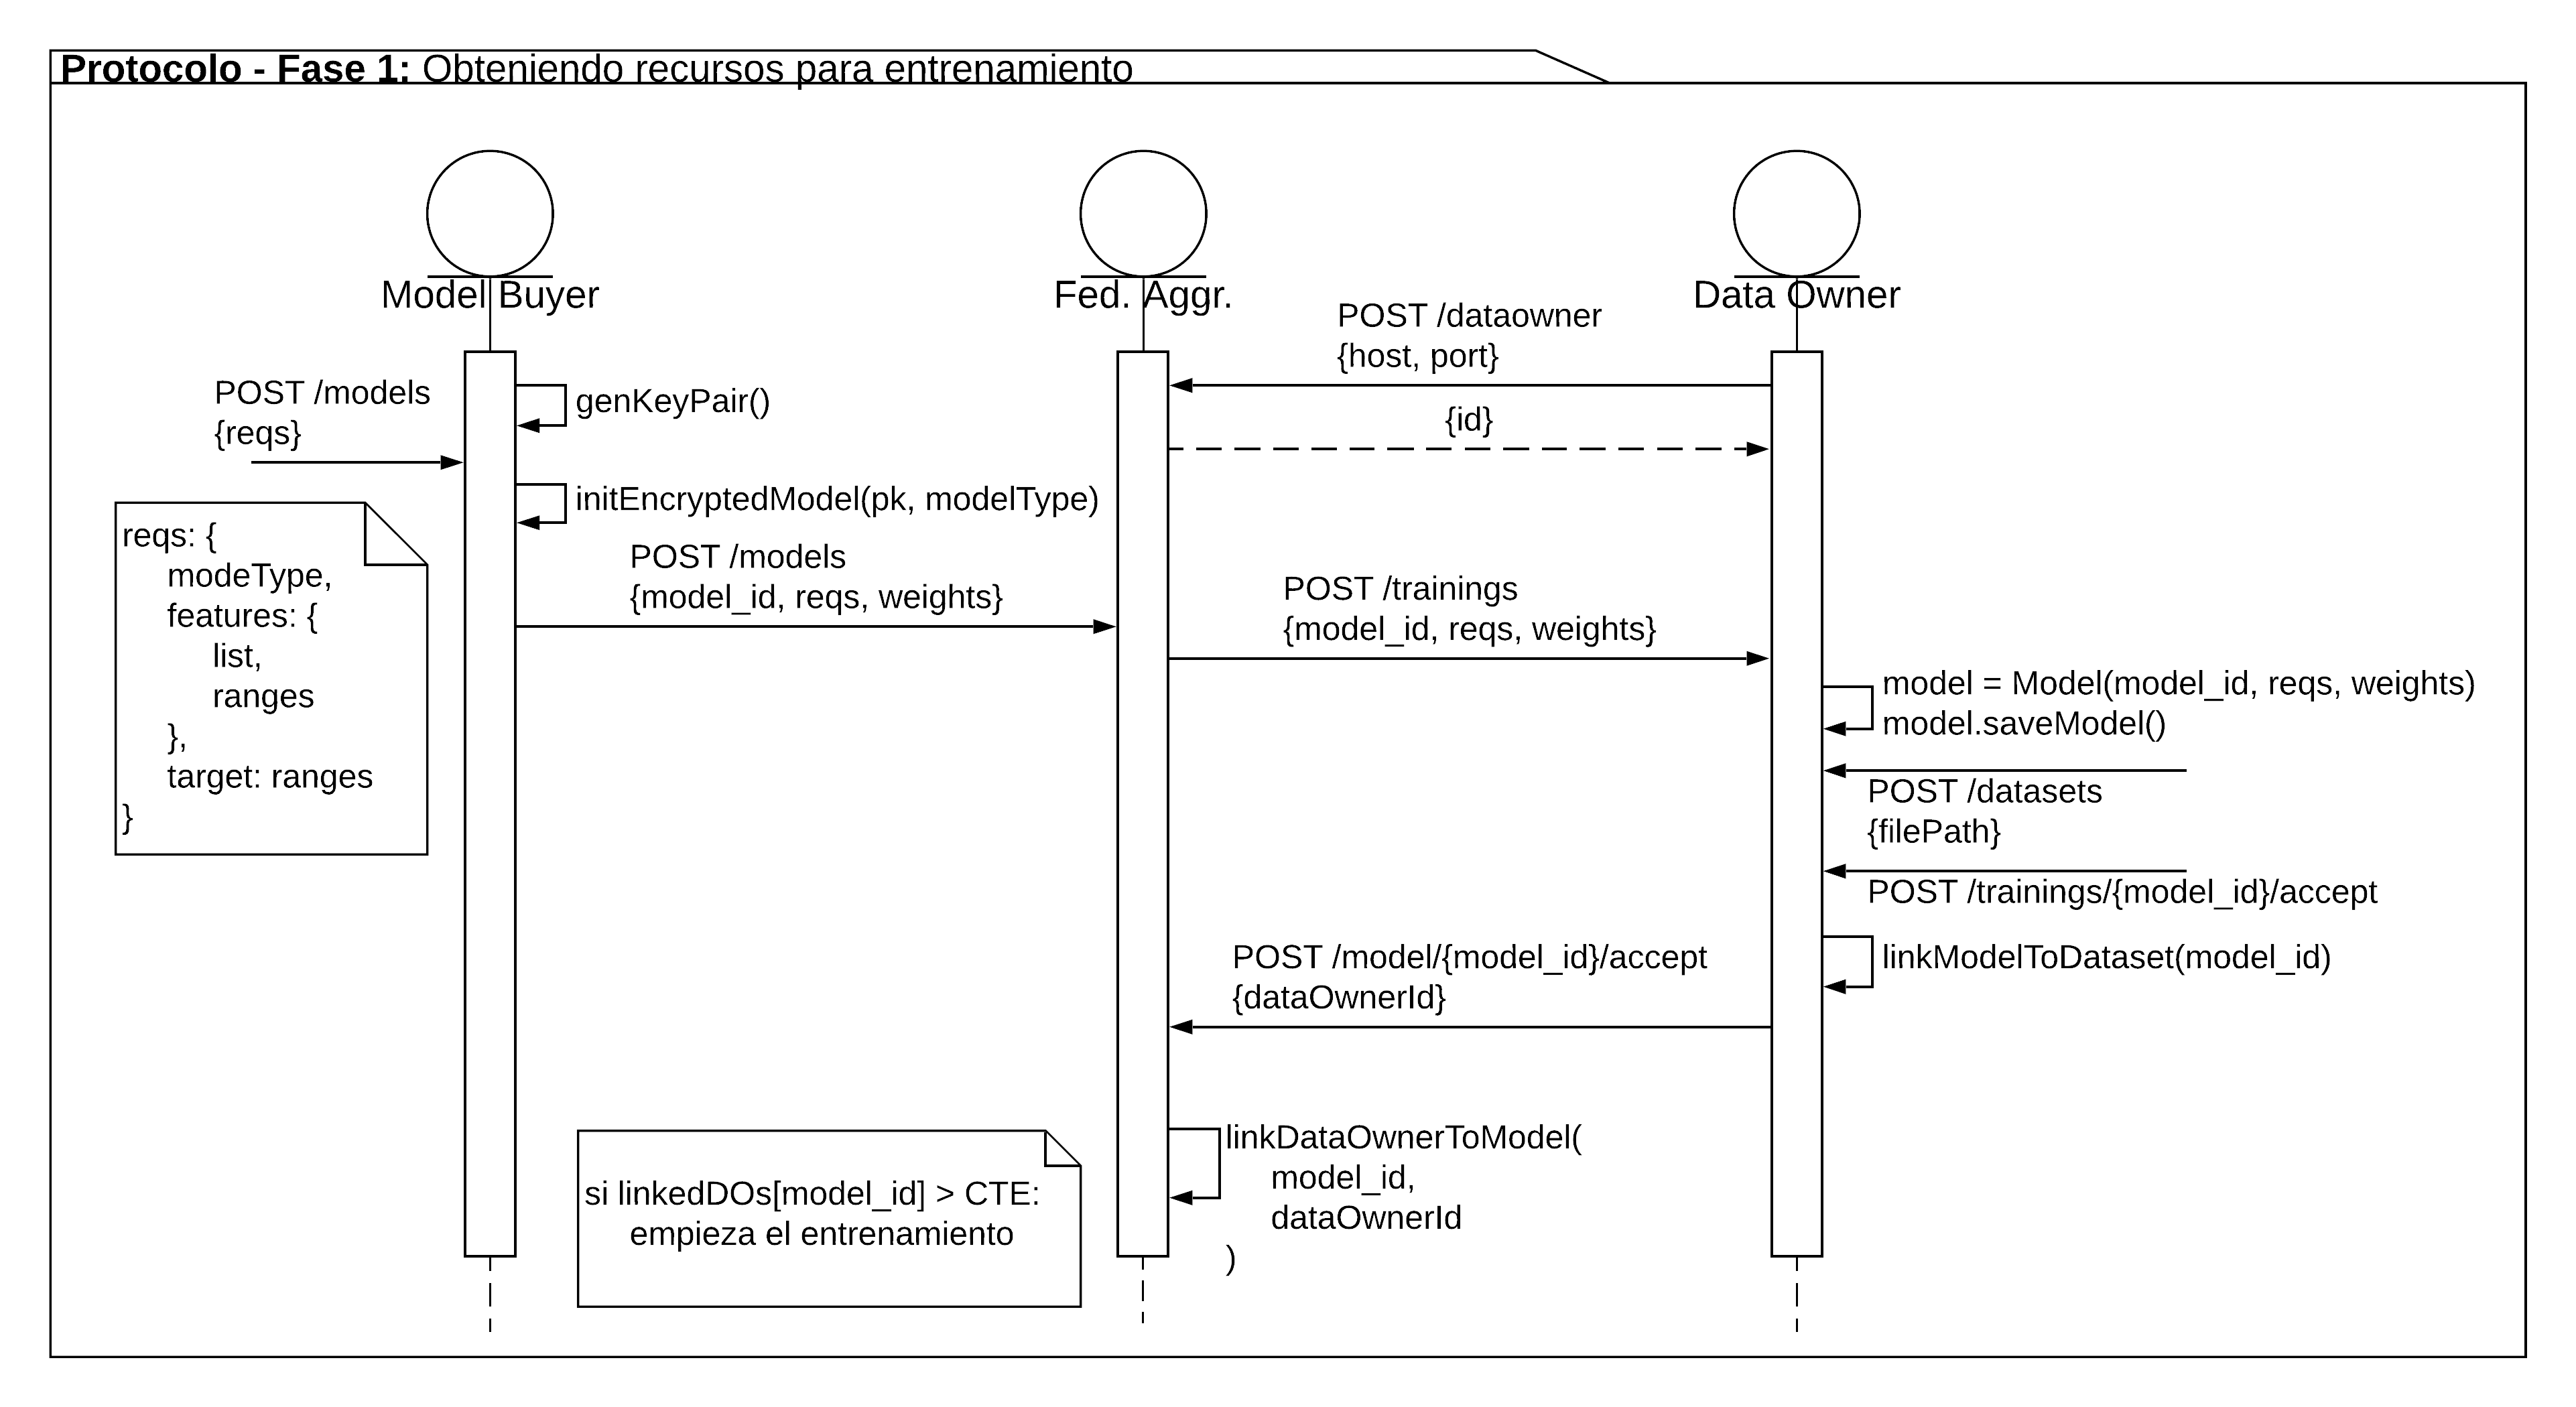
\includegraphics[scale=0.1]{imgs/flujo_fase1.png}
	\caption{Protocolo de inicialización del proceso de entrenamiento.}
\end{figure}

\subsection*{Entrenamiento del modelo encriptado}

El protocolo de entrenamiento encriptado, basado en la técnica de Federated Learning, define como se dará éste entrenamiento de manera distribuida, con el modelo encriptado en todo momento y, con cada Data Owner brindando sus datos locales y poder de cómputo.

\begin{figure}[H]
  	\centering
	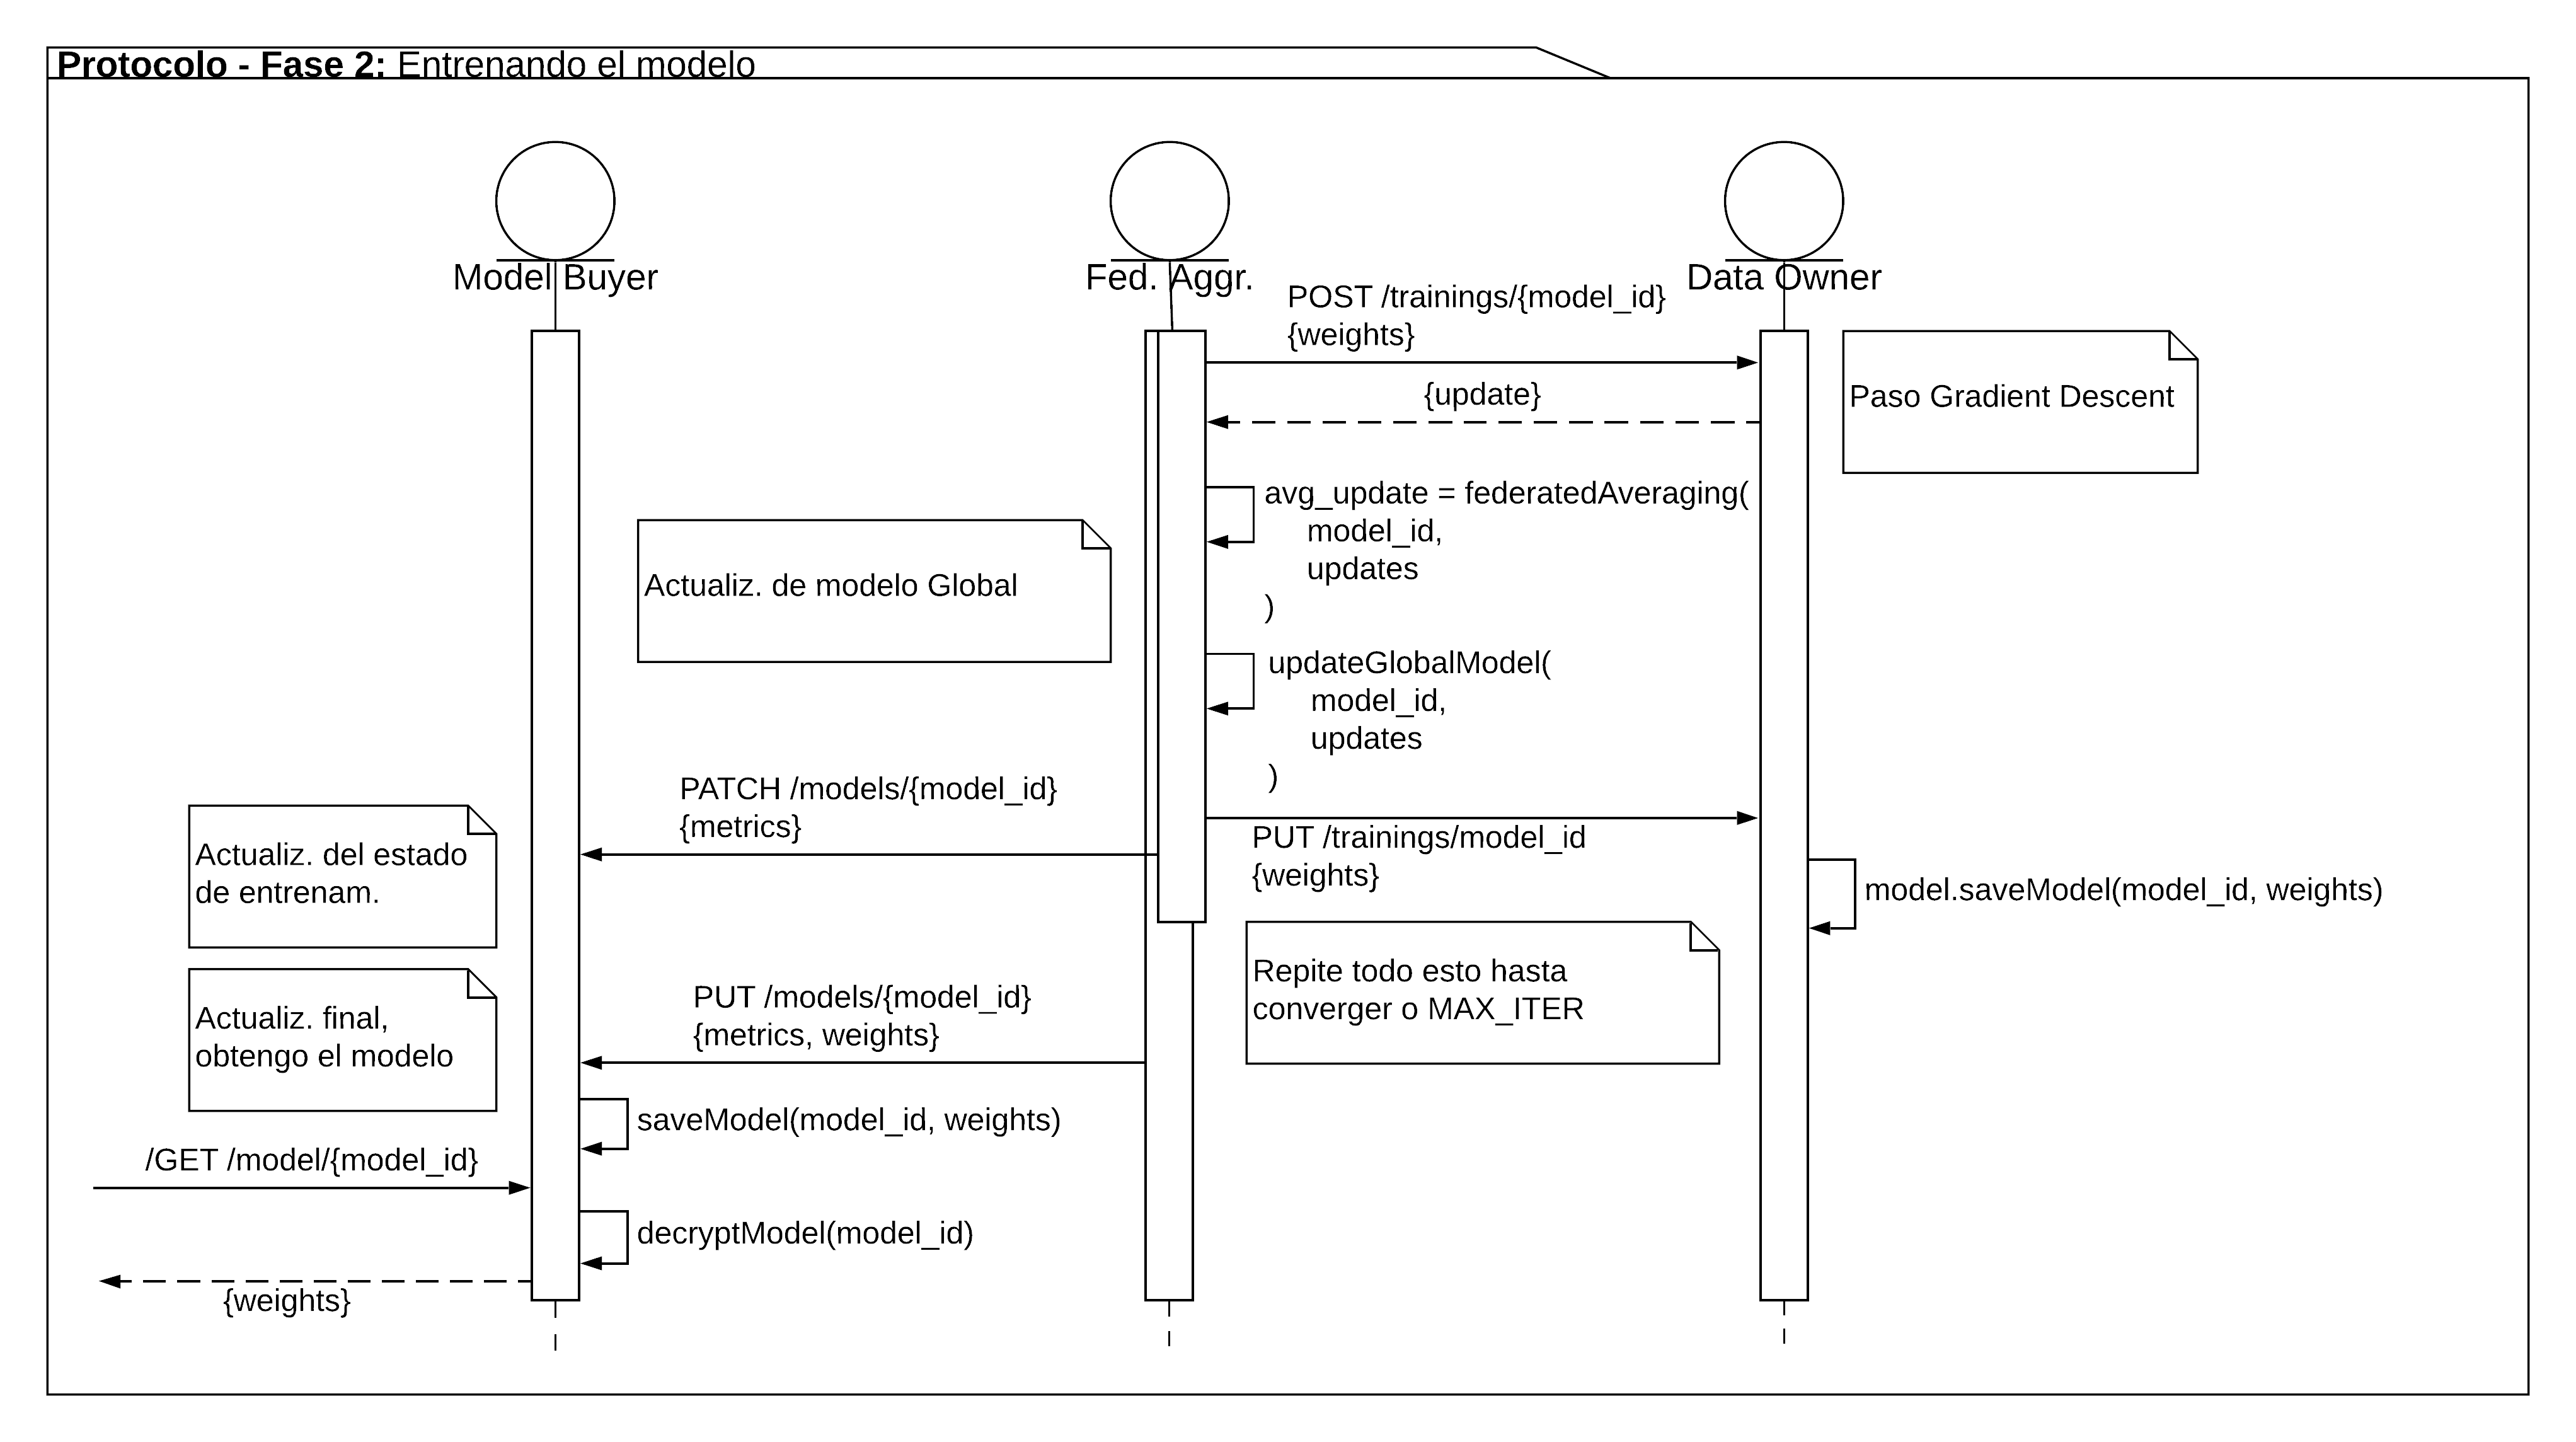
\includegraphics[scale=0.1]{imgs/flujo_fase2.png}
	\caption{Protocolo de entrenamiento de un modelo de manera distribuida y segura.}
\end{figure}

\subsection*{Calculo de métricas seguro}

El protocolo de calculo de métricas seguro fue creado debido a la incapacidad de los Data Owners en su rol de validador de calcular la métrica de calidad del modelo por ellos mismos. Ésta limitación existe dado que la biblitoca de Homomorphic Encryption utilizada no permite realizar productos entre números encriptados (y se necesita elevar un número encriptado al cuadrado para el calculo del MSE). Por lo que se ideó un protocolo mediante el cual, se puede computar el MSE sin que sea el Model Buyer quien lo haga (ya que podría alterar el calculo para obtener un beneficio), pero a la vez, dandole la posibilidad de validar dicho calculo.
El protocolo hace uso de una mecanica utilizada en Global Differential Privacy y en algunos esquemas de SMPC, la adición de ``ruido'' a la información que se envía a una parte en la que no se confía plenamente.

\begin{figure}[H]
  	\centering
	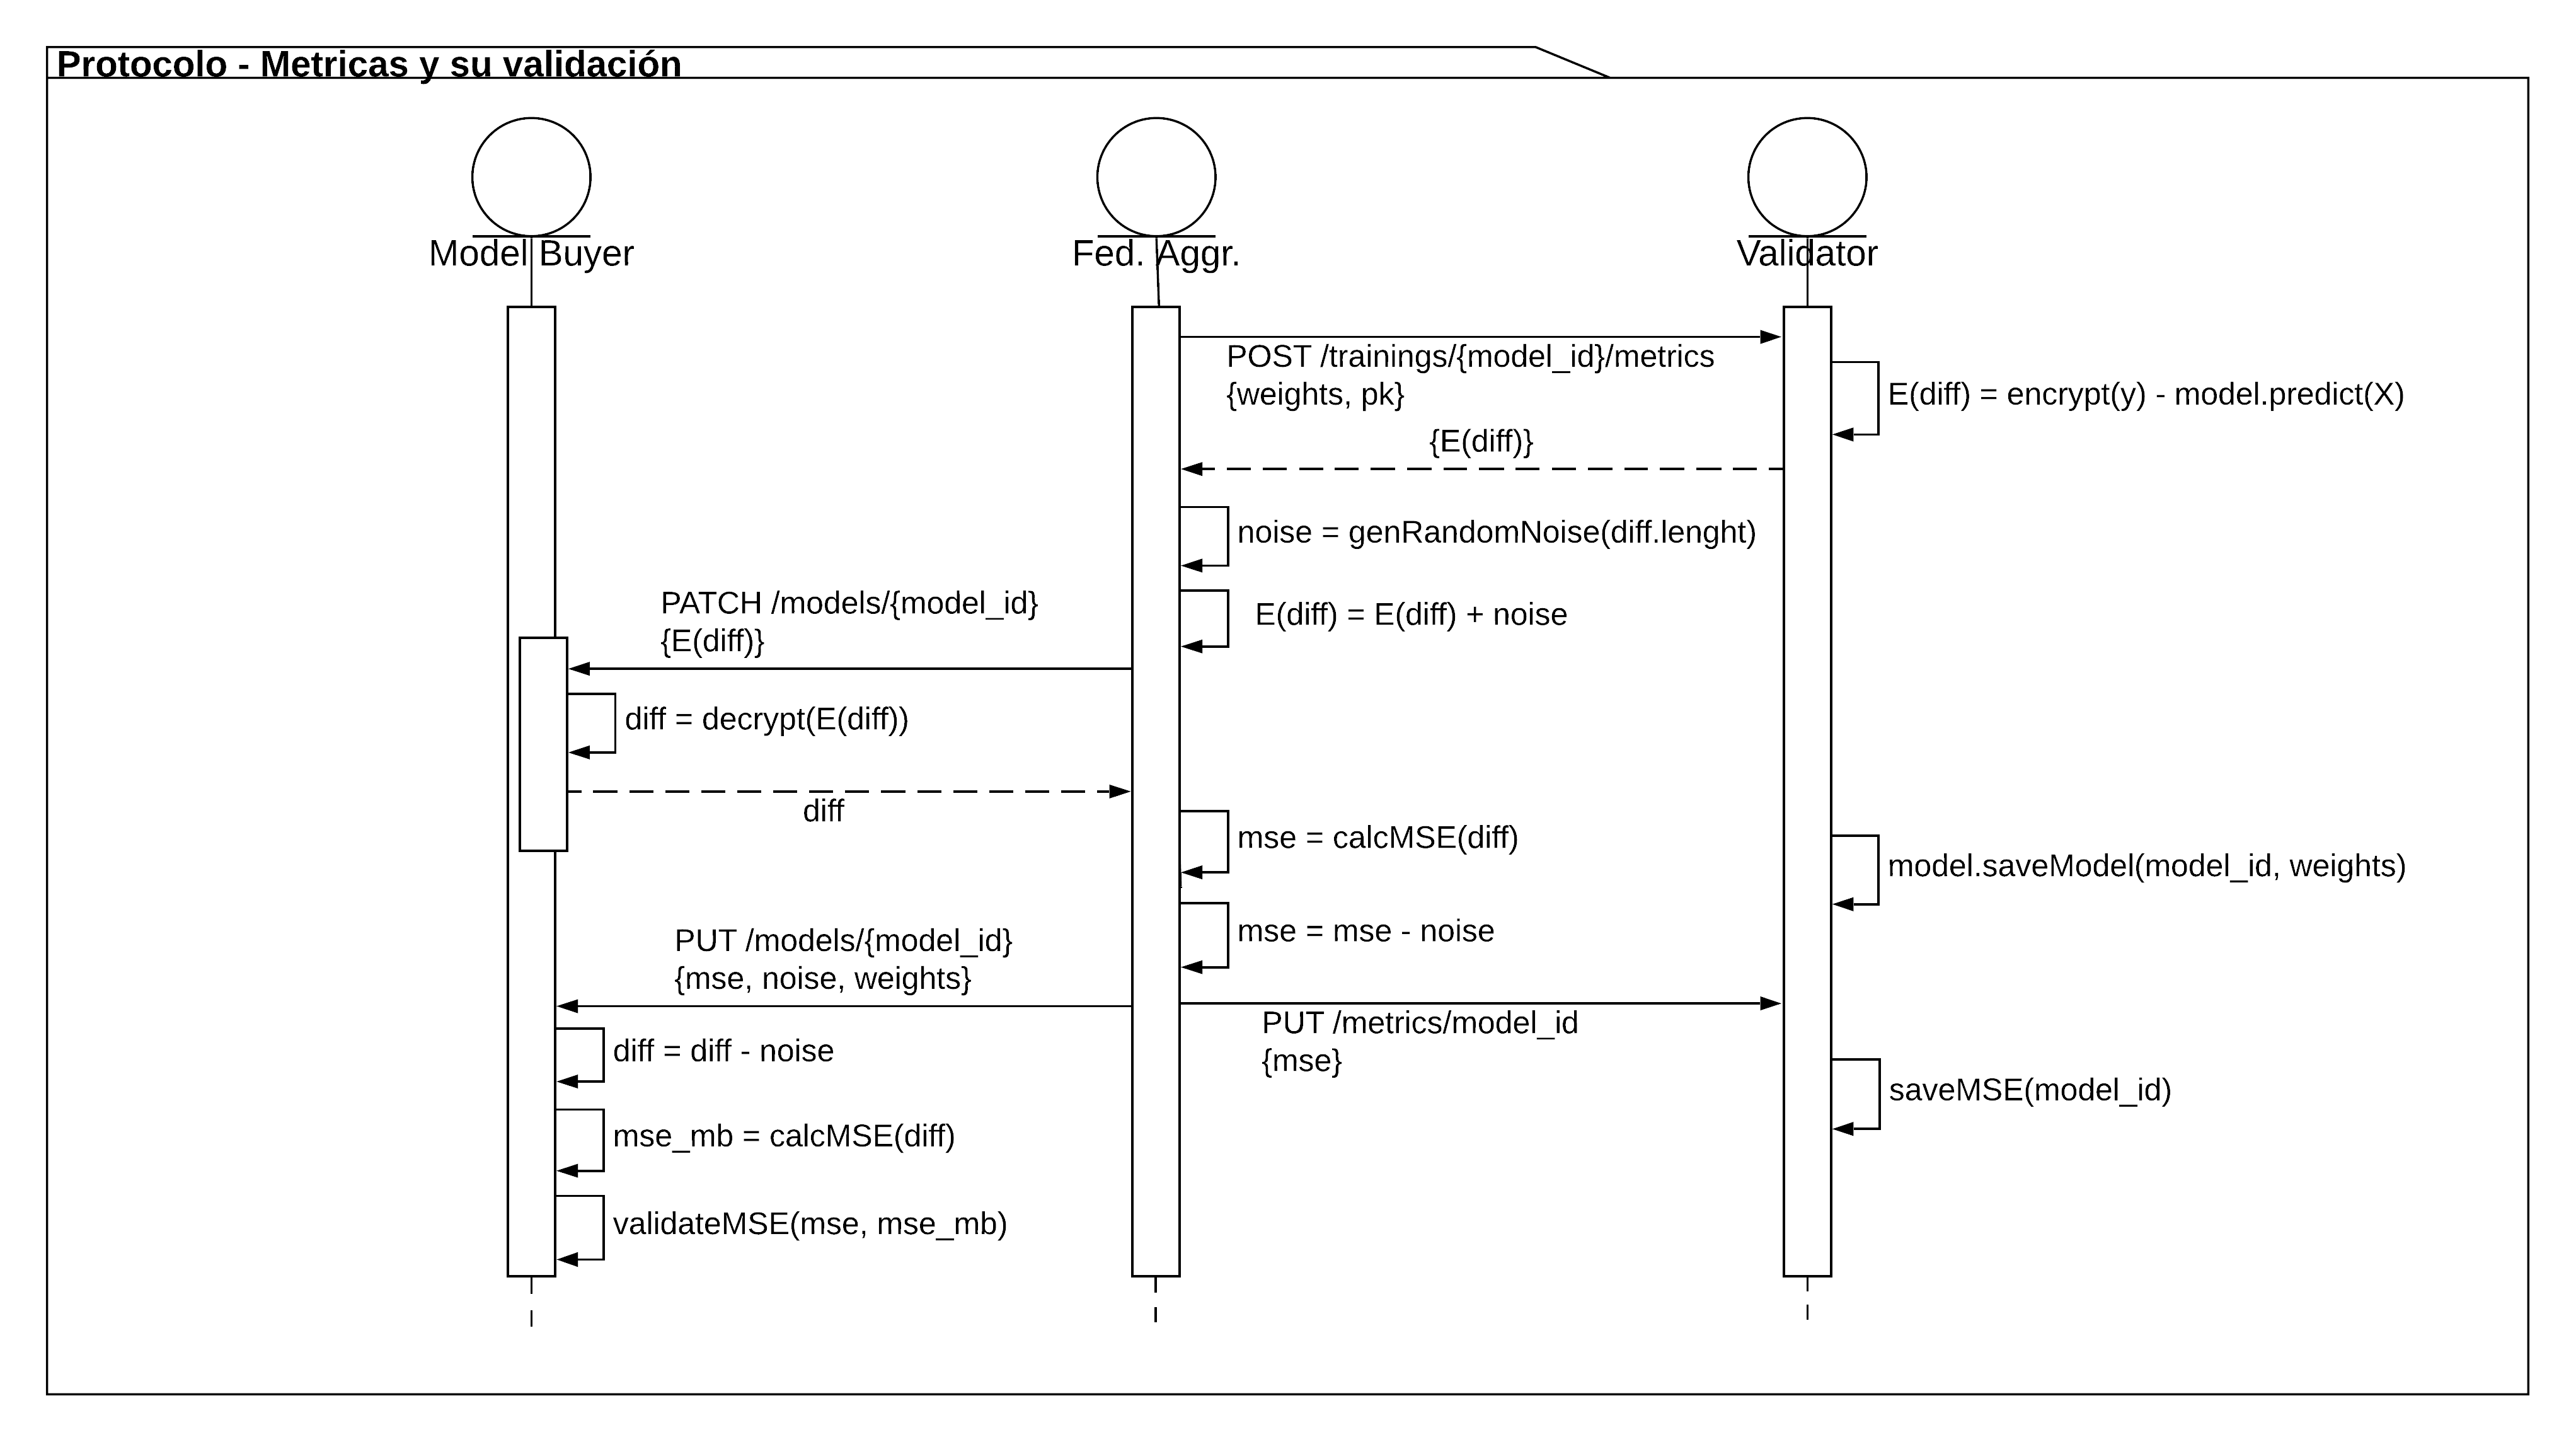
\includegraphics[scale=0.1]{imgs/flujo_valid.png}
	\caption{Esquema de calculo y validación de métricas seguro.}
	\label{fig:flujo_valid}
\end{figure}


\section{Imágenes de la plataforma DeltaML}

La figura \ref{fig:login} muestra la pantalla de Inicio de sesión que tanto el Data Owner como el Model Buyer ven antes de ingresar a la plataforma ingresando sus credenciales.

\begin{figure}[H]
  	\centering
	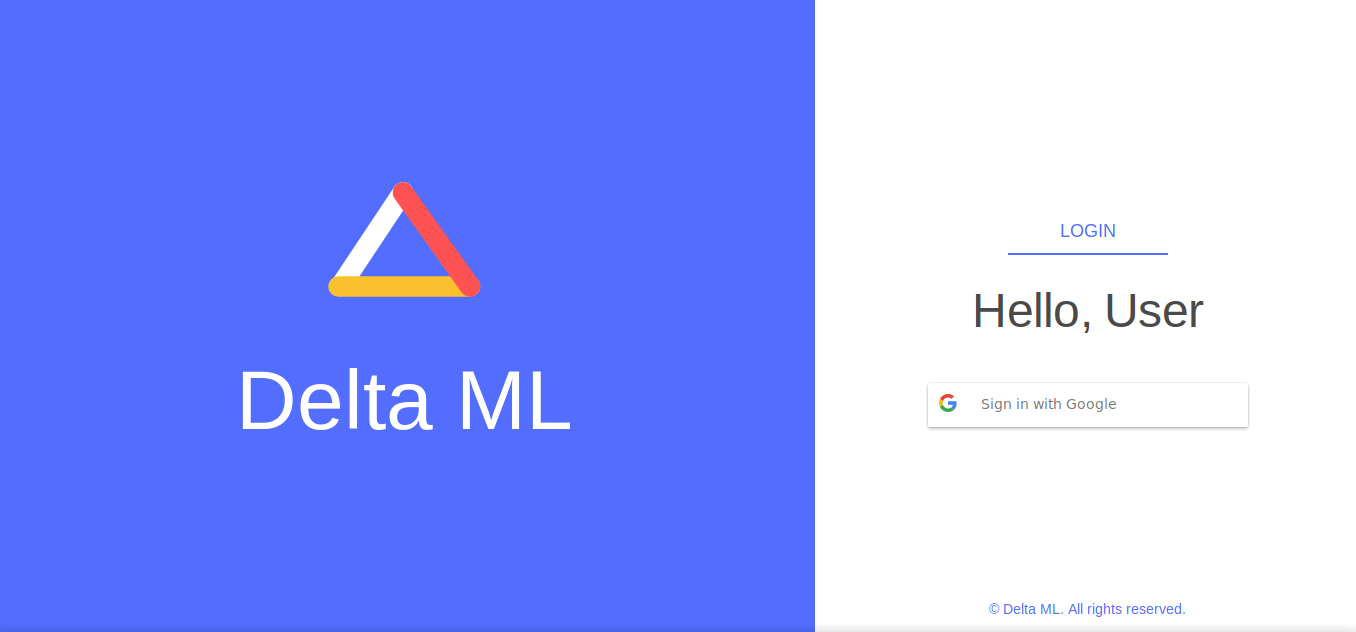
\includegraphics[scale=0.3]{imgs/Login.png}
	\caption{Pantalla de Login de la plataforma.}
	\label{fig:login}
\end{figure}

La figura \ref{fig:models_list} muestra la pantalla donde, el Data Owner puede ver todos los pedidos o solicitudes de entrenamiento de modelos que le han llegado. Estos pueden estar en los siguientes estados:

\begin{itemize}
\item \textbf{WAITING:} El Data Owner no tiene aún el dataset requerido para aceptar el entrenamiento. 
\item \textbf{READY:} El Data Owner tiene el dataset requerido pero no ha aceptado el entrenamiento aún. 
\item \textbf{INITIATED:} El Data Owner ha aceptado participar en el entrenamiento, pero el proceso no ha comenzado debido a que todavía no se ha alcanzado el número mínimo requerido de Data Owners que acepten la solicitud.
\item \textbf{IN PROGRESS:} El entrenamiento del modelo ha comenzado.
\item \textbf{FINISHED:} El entrenamiento del modelo finalizó. 
\end{itemize}

El Model Buyer tiene una pantalla similar pero para las solicitudes que realizó.

\begin{figure}[H]
  	\centering
	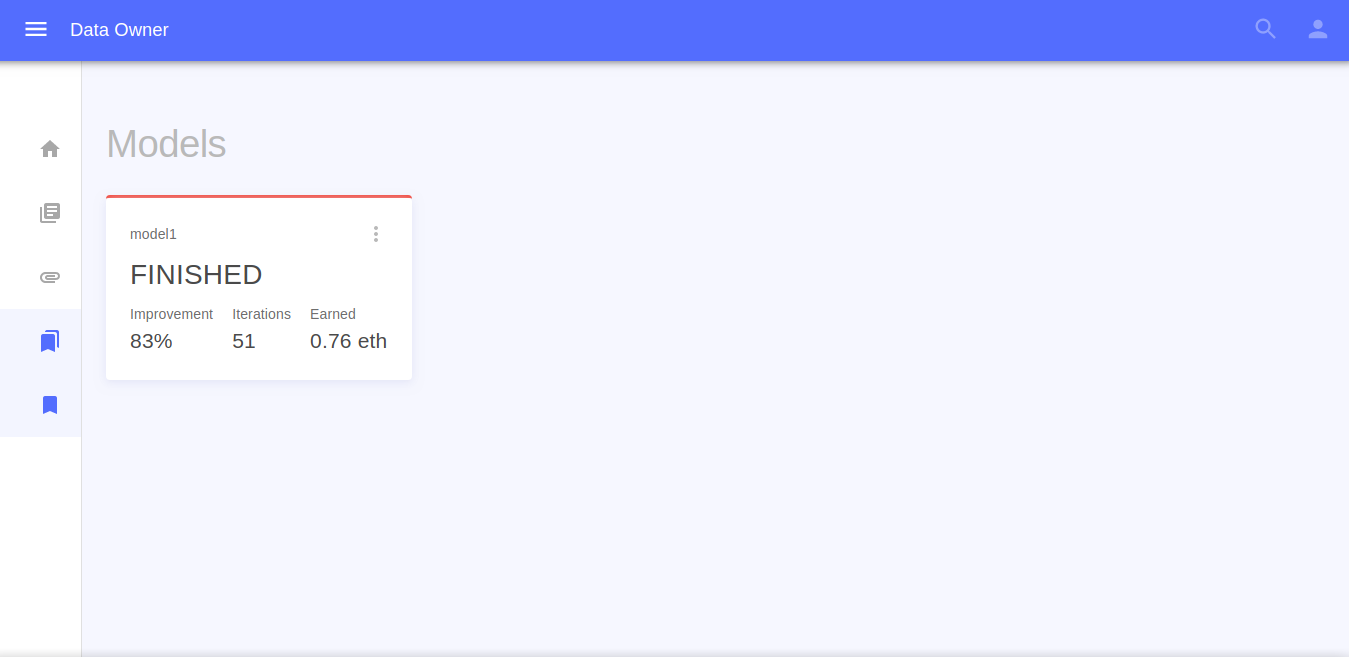
\includegraphics[scale=0.3]{imgs/ModelsList.png}
	\caption{Pantalla de lista entrenamientos solicitados al Data Owner.}
	\label{fig:models_list}
\end{figure}

La figura \ref{fig:model_progress} muestra la pantalla de detalle de progreso de un modelo en entrenamiento en el Model Buyer. En esta pantalla se puede observar el estado actual del modelo (los listados anteriormente), cuánto ha mejorado el modelo hasta ahora (expresado en porcentaje y a través de la métrica de calidad MSE) y cuánto se está pagando por el proceso hasta ahora.
Además se observa la progresión de la mejora del modelo en forma de grafico, donde la curva descendente es el MSE decreciendo hasta finalizar el entrenamiento. Y finalmente, se muestran las contribuciones que cada Data Owner en rol de entrenador realizaron al entrenamiento (expresado en porcentaje) y cuánto se le paga a cada uno por dicho trabajo.

\begin{figure}[H]
  	\centering
	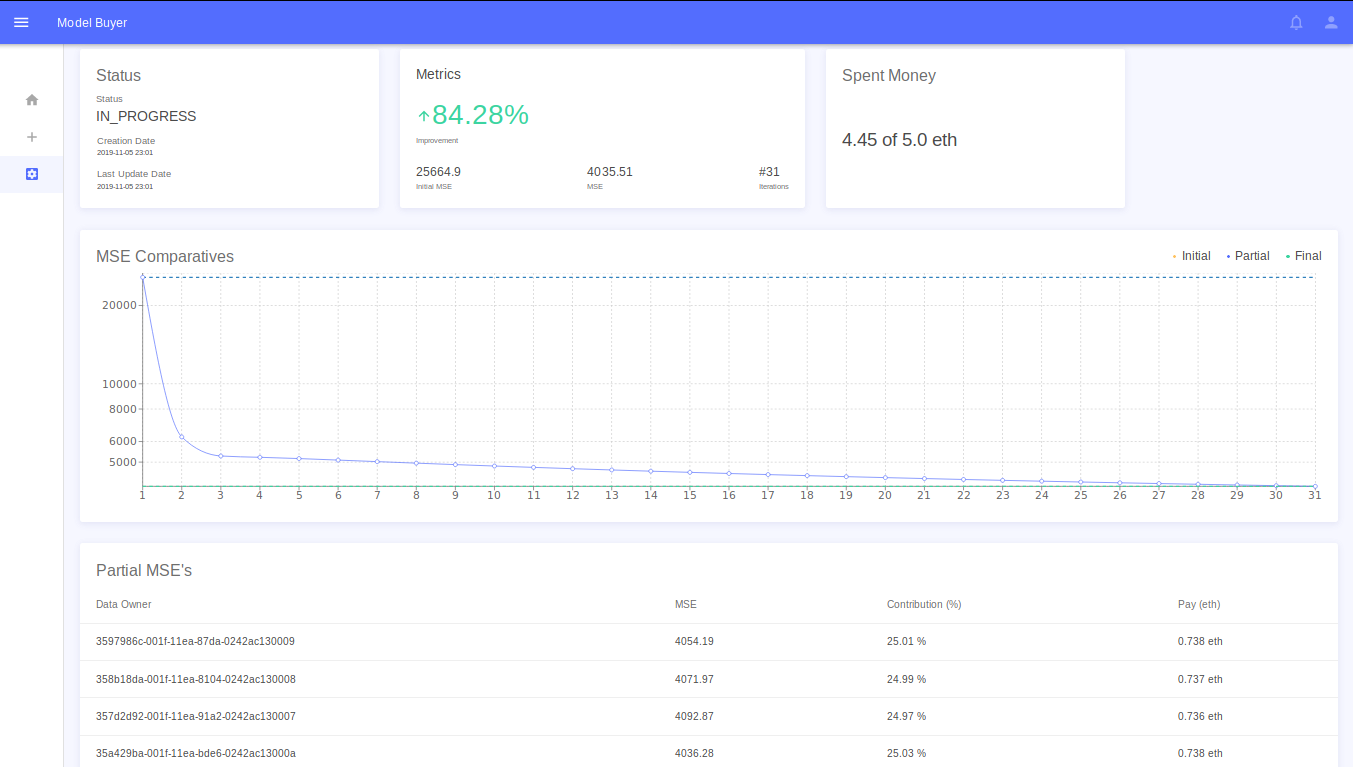
\includegraphics[scale=0.3]{imgs/ModelProgress.png}
	\caption{Pantalla de detalle del progreso del entrenamiento de un modelo en el ModelBuyer.}
	\label{fig:model_progress}
\end{figure}

\chapter{Resultados}

En el presente trabajo se desarrolló una plataforma capaz de entrenar modelos de manera descentralizada manteniendo la privacidad de los datos de los participantes involucrados. A su vez, se procuró que los modelos en entrenamiento no pudieran ser robados y ni tampoco las métricas alteradas. Todo esto se logró usando Homomorphic Encryption para generar un equema SMPC (Secure Multy-Party Computation), y Global Differential Privacy para el protocolo de calculo de métricas seguro.

Adicionalmente, se comparó la calidad del modelo entrenado usando el esquema implementado en el presente trabajo (con \textbf{5 Data Owners}) contra una regresión lineal tradicional. Para realizar ésta comparación se utilizaron los mismos datasets e hiperparametros, los cuales son:


\begin{itemize}
\item \textbf{Dataset:} Diabetes\cite{dataset} 
\item \textbf{Cantidad de iteraciones máxima:} 100
\item \textbf{Paso (Gradient Descent):} 1.5
\item \textbf{MSE Inicial (Modelo sin entrenar):} $\approx$ 27000
\end{itemize}

Y los resultados obtenidos fueron: \\

\begin{center}
\centering
\begin{tabular}{ || >{\centering\arraybackslash} p{6cm}| >{\centering\arraybackslash} p{6cm}||  }
 \hline
 \multicolumn{2}{|c|}{\textbf{MSE} (Mean Squared Error)} \\
 \hline\hline
 \textbf{DeltaML} & \textbf{Regresión Lineal local} \\
 \hline
 \rule{0pt}{4ex}  
 3311.84 & 3167.81 \\
 \hline
\end{tabular}
\end{center}

\bigskip

Por lo que, además de lo logrado en materia de privacidad y seguridad, el entrenamiento de los modelos por medio del esquema implementado continuó arrojando resultados similares a los de un entrenamiento tradicional con un dataset local.


\chapter{Trabajo futuro}
Dada la longitud del alcance del presente trabajo, algunas tareas fueron relegadas al no ser esenciales al objetivo planteado. Se detallan a continuación, algunos de los puntos que contemplamos como trabajo futuro para seguir profundizando sobre la temática de machine learning seguro y privado, o para continuar con el desarrollo de DeltaML: 
\begin{itemize}
\item Refactorizar el esquema para extraer un framework de Federated Leaning seguro y extensible tal que:

\begin{itemize}
\item El método de comunicación entre los participantes sea configurable (local, http, etc)
\item El mecanismo de SMPC sea extensible y se pueda cambiar por otro de manera simple.
\item Permita agregar nuevos tipos de modelo (regresión logística, redes neuronales, etc).
\item Pueda ser usado con varias bibliotecas de Machine Learning (como Scikit-learn, Spark ML o incluso Tensorflow).
\end{itemize}


\item Investigar otros métodos de SMPC y Homomorphic Encryption, y comparar como impacta uno u otro en la performance durante el entrenamiento de un modelo.
\item Migrar Data Owners a aplicaciones mobile.
\item Experimentar con otros frameworks (nuevos) de Federated Learning privado, tales como: PySift de OpenMined, TF-Encrypted de DropoutLabs, CrypTFlow de Microsoft.
\end{itemize}
 

\chapter{Conclusiones finales}
En este trabajo se propuso un esquema de entrenamiento de modelos de aprendizaje automático que no requieran el acceso físico a los datos por parte de quien desee entrenarlo, permitiendo preservar la privacidad de datos que quizas sean sensibles para los usuarios. A partir de esta propuesta se implementó DeltaML, plataforma que cumple con lo mencionado y, además, evita la apropiación del modelo en entrenamiento por cualquier otro participante de la misma. Como parte de esta solución se requería de una forma de pago a los distintos participantes que hubieran contribuido al entrenamiento. Sin embargo, usar un medio de pago que requiriera confiar en terceros, que centralizara esta dependencia o hiciera fácil algun tipo de fraude iba en contra del espiritú del trabajo. Por lo que se decidió optar por la plataforma Ethereum, que por medio de sus smart contract y el carácter descentralizado de su tecnología base brindaba todas las medidas de seguridad que un trabajo de estas caracteristicas requería.

En lo referente a los modelos de aprendizaje automático disponibles para entrenar por medio de DeltaML, por el momento está limitado a los de Regresión Lineal. Se optó por esta restricción para no ampliar el alcance del trabajo más allá de lo estipulado para un Trabajo Profesional de Ingeniería. Sin embargo, el proyecto es facilmente extendible para modelos de clasificación mediante Regresión Logística. El único punto a tener en cuenta, en ese caso, es que se deberá usar una aproximación de la función Sigmoide (si se optara por ésta), ya que la biblioteca de Homomorphic Encryption utilizada en el proyecto no permite operaciones no lineales entre números encriptados.

Con respecto a la performance, existe una diferencia considerable entre los tiempos entrenando un modelo usando DeltaML y usando un técnica tradicional. La plataforma desarrollada en el presente trabajo requiere de aproximadamente 15 minutos para entrenar el mismo modelo que de otra manera se logra entrenar en cuestión de segundos. Esta diferencia tan grande se debe a que todos los cálculos se dan sobre datos que se encuentran encriptados. Una mejora propuesta para disminuir esta baja de performance, es cambiar el mecanismo de SMPC actual (que usa Homomorphic Encryption) a uno como SPDZ \citep{spdz-1} \citep{spdz-2} \cite{spdz-prot} \cite{mpc-spdz}. 

Finalmente, la calidad de los modelos entrenados bajo la plataforma, en comparación con la de uno entrenado localmente utilizando una Regresión Lineal, no demuestra una disminución significativa. Por lo que al usar la plataforma se gana en protección de la privacidad y no se ve afectado el resultado final.


%----------------------------------------------------------------------------------------
%	BIBLIOGRAPHY
%----------------------------------------------------------------------------------------

\printbibliography[heading=bibnumbered, title=Referencias]

%----------------------------------------------------------------------------------------
%	GLOSARY
%----------------------------------------------------------------------------------------

\chapter{Glosario}
\begin{itemize}
\item \textbf{Machine Learning}: (en castellano Aprendizaje Automático) es la rama del área de la inteligencia artificial centrada en el estudio y construcción de sistemas capaces de aprender de los datos, identificar patrones y realizar decisiones con mínima intervención humana. 
\item \textbf{Deep Learning}: (o Aprendizaje Profundo) es un subconjunto del área de Machine Learning que intenta generar modelos que constan de arquitecturas compuestas de transformaciones no lineales múltiples. Se utilizan, en general, para resolver problemas de gran complejidad computacional por medio de aproximaciones logradas a través del entrenamiento de un modelo con las caracteristicas antes nombradas a partir de una cantidad enorme de datos.
\item \textbf{Blockchain}: o DLT (Descentralized Ledger Technology), es una tecnología que consta de un registro contable distribuido en una red de nodos. Las características principales de Blockchain son: inmutabilidad de la historia de las transacciones realizadas, resistencia a fraudes utilizando algoritmos de consenso entre los nodos de la red, transparencia (todos los nodos pueden ver el historial de transacciones), resistente a ataques (mediante la descentralización de los datos y el poder de computo combinado de todos los nodos participantes), y pseudo-anonimidad de los participantes de la red (se identifican con una clave que lleva el nombre de wallet, pero a  priori no hay forma de relacionar dicha wallet con su dueño).
\item \textbf{Smart Contract}: aplicaciones que se ejecutan sobre la red de nodos de una blockchain exactamente como fueron programadas sin ninguna posibilidad de downtime, censura, fraude o interferencia de una tercera parte.
\item \textbf{Differential Privacy}: es una técnica estadística que trata de maximizar la exactitud de la información que se desea obtener de una base de datos, mientras se minimiza el impacto  en la privacidad de las personas cuyos datos se encuentran en dicha base.
\item \textbf{Multi-party computation}: es una rama de la criptografía, la cual tiene por objetivo la creación de métodos para que diferentes partes puedan en conjunto realizar el computo de una función sobre sus datos a la vez que mantienen la privacidad de ellos.
\item \textbf{Homomorphic Encryption}: es un método de encriptación que difiere de los métodos típicos en que permite realizar cálculos directamente en datos encriptados sin requerir acceso a la clave. El resultado de tal cálculo permanece en forma encriptada, y puede ser revelado posteriormente por el propietario de la clave.
\end{itemize}


%----------------------------------------------------------------------------------------

\chapter{Tenologías utilizadas}

\section*{Homomorphic Encryption}

\subsection*{Python-paillier \cite{python-paillier}}
Biblioteca de python para Encriptación Homomórfica Parcial (Partially Homomorphic Encryption) basada en el cripto sistema Paillier \cite{paillier}. Se optó por esta biblioteca por las facilidades para serialización y deserialización de números encriptados que brinda.  

\section*{Blockchain}

\subsection*{Ethereum network \cite{eth}}
Plataforma descentralizada que ejecuta contratos inteligentes (smart contracts): aplicaciones que se ejecutan exactamente como fueron programadas sin ninguna posibilidad de downtime, censura, fraude o interferencia de una tercera parte.

\subsection*{Solidity \cite{sol}}
Lenguaje de alto nivel, orientado a objetos para implementar smart contracts. Los smart contracts son programas que gobiernan el comportamiento de cuentas dentro del ecosistema Ethereum.

\subsection*{Truffle \cite{tr}}
Framework de desarrollo de smart contracts para blockchains que utilizan la Máquina Virtual Ethereum (EVM).

\subsection*{Ganache \cite{gch}}
Blockchain personal para el desarrollo en Ethereum (testnet local) que se puede utilizar para implementar contratos, desarrollar sus aplicaciones y ejecutar pruebas.


\section*{API}

\subsection*{Python \cite{py}}
Lenguaje de alto nivel y tipado dinámico con soporte de paradigma de objetos que se utilizó para el desarrollo de los módulos de Federated Learning y Encriptación. Se eligió este lenguaje por su uso simple, por las herramientas desarrolladas para las áreas de Machine Learning y análisis de datos, y su gran adopción en el mundo del desarrollo y ciencias de datos, lo que reduce, también, dificultades en la resolución de problemas que puedan surgir durante el proyecto.

\subsection*{Flask \cite{flask}}
Flask es un framework minimalista escrito en Python que te permite crear aplicaciones web rápidamente y con un mínimo número de líneas de código.

\section*{UI}

\subsection*{React \cite{rt}}
Biblioteca Javascript de código abierto diseñada para crear interfaces de usuario con el objetivo de facilitar el desarrollo de aplicaciones en una sola página.

\section*{General}

\subsection*{Docker \cite{docker}}
Automatiza el despliegue de aplicaciones dentro de contenedores, proporcionando una capa adicional de abstracción y automatización de virtualización de aplicaciones en múltiples sistemas operativos.

\subsection*{Docker Compose \cite{docker-compose}}
Es una herramienta para definir y ejecutar aplicaciones que consisten en varios contendores de Docker.


%----------------------------------------------------------------------------------------

\chapter{Código fuente}

\begin{itemize}
\item \textbf{Model Buyer API:} \url{https://github.com/DeltaML/model-buyer}
\item \textbf{Model Buyer UI:} \url{https://github.com/DeltaML/model-buyer-ui}
\item \textbf{Data Owner API:} \url{https://github.com/DeltaML/data-owner}
\item \textbf{Data Owner UI:} \url{https://github.com/DeltaML/data-owner} 
\item \textbf{Federated Aggregator:} \url{https://github.com/DeltaML/federated-aggregator}
\item \textbf{Contract:} \url{https://github.com/DeltaML/contract}
\item \textbf{Libreria commons:} \url{https://github.com/DeltaML/commons}
\item \textbf{docker-compose:} \url{https://github.com/DeltaML/docker-compose}
\item \textbf{Scripts:} \url{https://github.com/DeltaML/testing}
\end{itemize}




%----------------------------------------------------------------------------------------

\end{document}  
